\documentclass[twoside]{book}

% Packages required by doxygen
\usepackage{fixltx2e}
\usepackage{calc}
\usepackage{doxygen}
\usepackage[export]{adjustbox} % also loads graphicx
\usepackage{graphicx}
\usepackage[utf8]{inputenc}
\usepackage{makeidx}
\usepackage{multicol}
\usepackage{multirow}
\PassOptionsToPackage{warn}{textcomp}
\usepackage{textcomp}
\usepackage[nointegrals]{wasysym}
\usepackage[table]{xcolor}

% Font selection
\usepackage[T1]{fontenc}
\usepackage[scaled=.90]{helvet}
\usepackage{courier}
\usepackage{amssymb}
\usepackage{sectsty}
\renewcommand{\familydefault}{\sfdefault}
\allsectionsfont{%
  \fontseries{bc}\selectfont%
  \color{darkgray}%
}
\renewcommand{\DoxyLabelFont}{%
  \fontseries{bc}\selectfont%
  \color{darkgray}%
}
\newcommand{\+}{\discretionary{\mbox{\scriptsize$\hookleftarrow$}}{}{}}

% Page & text layout
\usepackage{geometry}
\geometry{%
  a4paper,%
  top=2.5cm,%
  bottom=2.5cm,%
  left=2.5cm,%
  right=2.5cm%
}
\tolerance=750
\hfuzz=15pt
\hbadness=750
\setlength{\emergencystretch}{15pt}
\setlength{\parindent}{0cm}
\setlength{\parskip}{3ex plus 2ex minus 2ex}
\makeatletter
\renewcommand{\paragraph}{%
  \@startsection{paragraph}{4}{0ex}{-1.0ex}{1.0ex}{%
    \normalfont\normalsize\bfseries\SS@parafont%
  }%
}
\renewcommand{\subparagraph}{%
  \@startsection{subparagraph}{5}{0ex}{-1.0ex}{1.0ex}{%
    \normalfont\normalsize\bfseries\SS@subparafont%
  }%
}
\makeatother

% Headers & footers
\usepackage{fancyhdr}
\pagestyle{fancyplain}
\fancyhead[LE]{\fancyplain{}{\bfseries\thepage}}
\fancyhead[CE]{\fancyplain{}{}}
\fancyhead[RE]{\fancyplain{}{\bfseries\leftmark}}
\fancyhead[LO]{\fancyplain{}{\bfseries\rightmark}}
\fancyhead[CO]{\fancyplain{}{}}
\fancyhead[RO]{\fancyplain{}{\bfseries\thepage}}
\fancyfoot[LE]{\fancyplain{}{}}
\fancyfoot[CE]{\fancyplain{}{}}
\fancyfoot[RE]{\fancyplain{}{\bfseries\scriptsize Generated by Doxygen }}
\fancyfoot[LO]{\fancyplain{}{\bfseries\scriptsize Generated by Doxygen }}
\fancyfoot[CO]{\fancyplain{}{}}
\fancyfoot[RO]{\fancyplain{}{}}
\renewcommand{\footrulewidth}{0.4pt}
\renewcommand{\chaptermark}[1]{%
  \markboth{#1}{}%
}
\renewcommand{\sectionmark}[1]{%
  \markright{\thesection\ #1}%
}

% Indices & bibliography
\usepackage{natbib}
\usepackage[titles]{tocloft}
\setcounter{tocdepth}{3}
\setcounter{secnumdepth}{5}
\makeindex

% Hyperlinks (required, but should be loaded last)
\usepackage{ifpdf}
\ifpdf
  \usepackage[pdftex,pagebackref=true]{hyperref}
\else
  \usepackage[ps2pdf,pagebackref=true]{hyperref}
\fi
\hypersetup{%
  colorlinks=true,%
  linkcolor=blue,%
  citecolor=blue,%
  unicode%
}

% Custom commands
\newcommand{\clearemptydoublepage}{%
  \newpage{\pagestyle{empty}\cleardoublepage}%
}

\usepackage{caption}
\captionsetup{labelsep=space,justification=centering,font={bf},singlelinecheck=off,skip=4pt,position=top}

%===== C O N T E N T S =====

\begin{document}

% Titlepage & ToC
\hypersetup{pageanchor=false,
             bookmarksnumbered=true,
             pdfencoding=unicode
            }
\pagenumbering{alph}
\begin{titlepage}
\vspace*{7cm}
\begin{center}%
{\Large B\+M\+P280 TivaC Driver }\\
\vspace*{1cm}
{\large Generated by Doxygen 1.8.13}\\
\end{center}
\end{titlepage}
\clearemptydoublepage
\pagenumbering{roman}
\tableofcontents
\clearemptydoublepage
\pagenumbering{arabic}
\hypersetup{pageanchor=true}

%--- Begin generated contents ---
\chapter{B\+M\+P280 Driver using TivaC}
\label{index}\hypertarget{index}{}Library used for interacting the bmp280 with tivaC tm4c123gh6pm processor, the dev board used is the TivaC line of Texas Instrument

The bmp280 board used is from Adafruit\+: \href{https://www.adafruit.com/product/2651}{\tt https\+://www.\+adafruit.\+com/product/2651}

Some A\+PI for compensating and collecting raw data was borrowed from Bosch\+: \href{https://github.com/BoschSensortec/BMP280_driver}{\tt https\+://github.\+com/\+Bosch\+Sensortec/\+B\+M\+P280\+\_\+driver}

The project was developed using Segger Embedded Studio but you should be able to use other I\+DE or build system with it

\subsection*{Features}


\begin{DoxyItemize}
\item Read and calculate compensated temperature and pressure data
\item Read and write settings
\item Read the status of the sensor
\item Create manufacturer-\/defined settings or custom settings
\item Available in both I2C and S\+PI
\end{DoxyItemize}

\subsection*{Dependencies}

The dependency is in the form of the git submodules of one of my other repo, just initialize and pull that sub module and you should be good, you can also write your own

\subsection*{Folder structure}


\begin{DoxyItemize}
\item src/\+: driver .c files in here
\item include/\+: .h file here
\item external/\+: Dependencies go here, for example git submodules are here
\item docs/\+: doxygen generated docs
\end{DoxyItemize}

\subsection*{Code structure}

The code is divided into many layers\+:


\begin{DoxyItemize}
\item B\+M\+P280\+\_\+\+Drv files\+: the front layers, their actions are B\+M\+P280 specifc but doesn\textquotesingle{}t deal directly with S\+PI or I2C and thus agnostic to the protocol
\item B\+M\+P280\+\_\+\+Ware files\+: contain A\+PI derived from Bosch source code
\item B\+M\+P280\+\_\+\+Utils\+: contain utilities functions for B\+M\+P280\+\_\+\+Drv as well as dealing directly with the I2C and S\+PI, this is the glue layer between B\+M\+P280\+\_\+\+Drv and low layer communication functions
\item Tiva\+C\+\_\+\+S\+PI related files\+: Contain S\+PI functions for S\+P\+I0 modules of TivaC, the code is hardocded to use module 0, the CS pin hardcoded to be pin 3 of port A on the TivaC board
\item Tiva\+C\+\_\+\+I2C related files\+: Contain TivaC functions and their utilities funcs to work with I2\+C0 modules of TivaC, hard coded to use I2\+C0 
\end{DoxyItemize}
\chapter{Data Structure Index}
\section{Data Structures}
Here are the data structures with brief descriptions\+:\begin{DoxyCompactList}
\item\contentsline{section}{\hyperlink{structBmp280CalibParam}{Bmp280\+Calib\+Param} \\*Calibration data struct }{\pageref{structBmp280CalibParam}}{}
\item\contentsline{section}{\hyperlink{structbmp280Sensor}{bmp280\+Sensor} \\*Data structure of a bmp280 }{\pageref{structbmp280Sensor}}{}
\item\contentsline{section}{\hyperlink{structBmp280Status}{Bmp280\+Status} \\*Indicate status of the bmp280 }{\pageref{structBmp280Status}}{}
\item\contentsline{section}{\hyperlink{structSpiSettings}{Spi\+Settings} \\*Represent a spi module }{\pageref{structSpiSettings}}{}
\end{DoxyCompactList}

\chapter{File Index}
\section{File List}
Here is a list of all documented files with brief descriptions\+:\begin{DoxyCompactList}
\item\contentsline{section}{include/\hyperlink{BMP280__Drv_8h}{B\+M\+P280\+\_\+\+Drv.\+h} \\*Contain data structures for B\+M\+P280 }{\pageref{BMP280__Drv_8h}}{}
\item\contentsline{section}{include/\hyperlink{BMP280__Utils_8h}{B\+M\+P280\+\_\+\+Utils.\+h} \\*Headers to B\+M\+P280 utils functions }{\pageref{BMP280__Utils_8h}}{}
\item\contentsline{section}{include/\hyperlink{BMP280__Ware_8h}{B\+M\+P280\+\_\+\+Ware.\+h} \\*Utils header that contain Bosch data structure for calibration data as well as bit positions of data }{\pageref{BMP280__Ware_8h}}{}
\item\contentsline{section}{include/\hyperlink{TivaC__I2C_8h}{Tiva\+C\+\_\+\+I2\+C.\+h} \\*Contain i2c error enum and function prototypes }{\pageref{TivaC__I2C_8h}}{}
\item\contentsline{section}{include/\hyperlink{TivaC__SPI_8h}{Tiva\+C\+\_\+\+S\+P\+I.\+h} \\*Contain data structure for S\+PI settings, errors as well as enum for various settings }{\pageref{TivaC__SPI_8h}}{}
\item\contentsline{section}{include/\hyperlink{TivaC__SPI__utils_8h}{Tiva\+C\+\_\+\+S\+P\+I\+\_\+utils.\+h} \\*Header file for S\+PI utilities functions }{\pageref{TivaC__SPI__utils_8h}}{}
\item\contentsline{section}{src/\hyperlink{BMP280__Drv_8c}{B\+M\+P280\+\_\+\+Drv.\+c} \\*Driver files, contain the top layer of the B\+M\+P280 A\+PI, contains ideally no I2C or S\+PI specific stuffs }{\pageref{BMP280__Drv_8c}}{}
\item\contentsline{section}{src/\hyperlink{BMP280__Utils_8c}{B\+M\+P280\+\_\+\+Utils.\+c} \\*Utils files contain helper functions for \hyperlink{BMP280__Drv_8c}{B\+M\+P280\+\_\+\+Drv.\+c} files as well as the glues to work with I2C and S\+PI specific stuffs }{\pageref{BMP280__Utils_8c}}{}
\item\contentsline{section}{src/\hyperlink{BMP280__Ware_8c}{B\+M\+P280\+\_\+\+Ware.\+c} \\*Contain A\+PI adapted from Bosch official source code }{\pageref{BMP280__Ware_8c}}{}
\item\contentsline{section}{src/\hyperlink{main_8c}{main.\+c} \\*Used for testing and also serve as an example }{\pageref{main_8c}}{}
\item\contentsline{section}{src/\hyperlink{TivaC__I2C_8c}{Tiva\+C\+\_\+\+I2\+C.\+c} \\*Contain main I2C functions for T\+IvaC }{\pageref{TivaC__I2C_8c}}{}
\end{DoxyCompactList}

\chapter{Data Structure Documentation}
\hypertarget{structBmp280CalibParam}{}\section{Bmp280\+Calib\+Param Struct Reference}
\label{structBmp280CalibParam}\index{Bmp280\+Calib\+Param@{Bmp280\+Calib\+Param}}


calibration data struct  




{\ttfamily \#include $<$B\+M\+P280\+\_\+\+Ware.\+h$>$}

\subsection*{Data Fields}
\begin{DoxyCompactItemize}
\item 
\mbox{\Hypertarget{structBmp280CalibParam_af0f31d919328127b19afc10185575f03}\label{structBmp280CalibParam_af0f31d919328127b19afc10185575f03}} 
uint16\+\_\+t {\bfseries dig\+\_\+t1}
\item 
\mbox{\Hypertarget{structBmp280CalibParam_a8dc60a38b57224e2917436127b3f42d3}\label{structBmp280CalibParam_a8dc60a38b57224e2917436127b3f42d3}} 
int16\+\_\+t {\bfseries dig\+\_\+t2}
\item 
\mbox{\Hypertarget{structBmp280CalibParam_aac8e49eec584c4097c805574ca02faa4}\label{structBmp280CalibParam_aac8e49eec584c4097c805574ca02faa4}} 
int16\+\_\+t {\bfseries dig\+\_\+t3}
\item 
\mbox{\Hypertarget{structBmp280CalibParam_a71a393a6e1285904df415ea278c43c19}\label{structBmp280CalibParam_a71a393a6e1285904df415ea278c43c19}} 
uint16\+\_\+t {\bfseries dig\+\_\+p1}
\item 
\mbox{\Hypertarget{structBmp280CalibParam_adeb9748540681fc42690052938b1bf96}\label{structBmp280CalibParam_adeb9748540681fc42690052938b1bf96}} 
int16\+\_\+t {\bfseries dig\+\_\+p2}
\item 
\mbox{\Hypertarget{structBmp280CalibParam_a08160ac14aa2c9fe485f6a40db273452}\label{structBmp280CalibParam_a08160ac14aa2c9fe485f6a40db273452}} 
int16\+\_\+t {\bfseries dig\+\_\+p3}
\item 
\mbox{\Hypertarget{structBmp280CalibParam_ab5c947d981b18daf5ecf0c5419a0cd50}\label{structBmp280CalibParam_ab5c947d981b18daf5ecf0c5419a0cd50}} 
int16\+\_\+t {\bfseries dig\+\_\+p4}
\item 
\mbox{\Hypertarget{structBmp280CalibParam_aa50f166ca650f984b80eb28df8edcd7b}\label{structBmp280CalibParam_aa50f166ca650f984b80eb28df8edcd7b}} 
int16\+\_\+t {\bfseries dig\+\_\+p5}
\item 
\mbox{\Hypertarget{structBmp280CalibParam_a60d948c94033428c6b749fdde12ae30f}\label{structBmp280CalibParam_a60d948c94033428c6b749fdde12ae30f}} 
int16\+\_\+t {\bfseries dig\+\_\+p6}
\item 
\mbox{\Hypertarget{structBmp280CalibParam_a6aa23c97e1323e8e4edfdb9b0d94a994}\label{structBmp280CalibParam_a6aa23c97e1323e8e4edfdb9b0d94a994}} 
int16\+\_\+t {\bfseries dig\+\_\+p7}
\item 
\mbox{\Hypertarget{structBmp280CalibParam_acc907ae1329f78c0fa8991ae02ed1608}\label{structBmp280CalibParam_acc907ae1329f78c0fa8991ae02ed1608}} 
int16\+\_\+t {\bfseries dig\+\_\+p8}
\item 
\mbox{\Hypertarget{structBmp280CalibParam_af43910766b70a48f4323b2fae0dee380}\label{structBmp280CalibParam_af43910766b70a48f4323b2fae0dee380}} 
int16\+\_\+t {\bfseries dig\+\_\+p9}
\item 
\mbox{\Hypertarget{structBmp280CalibParam_a2b264faa7220fc178a4a255252db43bc}\label{structBmp280CalibParam_a2b264faa7220fc178a4a255252db43bc}} 
int32\+\_\+t {\bfseries t\+\_\+fine}
\end{DoxyCompactItemize}


\subsection{Detailed Description}
calibration data struct 

The documentation for this struct was generated from the following file\+:\begin{DoxyCompactItemize}
\item 
include/\hyperlink{BMP280__Ware_8h}{B\+M\+P280\+\_\+\+Ware.\+h}\end{DoxyCompactItemize}

\hypertarget{structbmp280Sensor}{}\section{bmp280\+Sensor Struct Reference}
\label{structbmp280Sensor}\index{bmp280\+Sensor@{bmp280\+Sensor}}


data structure of a bmp280  




{\ttfamily \#include $<$B\+M\+P280\+\_\+\+Drv.\+h$>$}



Collaboration diagram for bmp280\+Sensor\+:\nopagebreak
\begin{figure}[H]
\begin{center}
\leavevmode
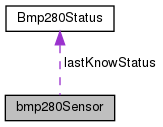
\includegraphics[width=194pt]{structbmp280Sensor__coll__graph}
\end{center}
\end{figure}
\subsection*{Data Fields}
\begin{DoxyCompactItemize}
\item 
\mbox{\Hypertarget{structbmp280Sensor_aba78f289019429a499ea47b952d03369}\label{structbmp280Sensor_aba78f289019429a499ea47b952d03369}} 
uint8\+\_\+t \hyperlink{structbmp280Sensor_aba78f289019429a499ea47b952d03369}{ID}
\begin{DoxyCompactList}\small\item\em $<$ protocol information \end{DoxyCompactList}\item 
\mbox{\Hypertarget{structbmp280Sensor_a5b65eb591144f9e09cc7b9695bd232d3}\label{structbmp280Sensor_a5b65eb591144f9e09cc7b9695bd232d3}} 
uint8\+\_\+t {\bfseries address}
\item 
\mbox{\Hypertarget{structbmp280Sensor_ade09526aa1ba4050e7240aa588e6f787}\label{structbmp280Sensor_ade09526aa1ba4050e7240aa588e6f787}} 
\hyperlink{BMP280__Drv_8h_ab4295e33e8c981aef15803030d176782}{Bmp280\+Com\+Protocol} \hyperlink{structbmp280Sensor_ade09526aa1ba4050e7240aa588e6f787}{protocol}
\begin{DoxyCompactList}\small\item\em oversampling settings \end{DoxyCompactList}\item 
\mbox{\Hypertarget{structbmp280Sensor_ab21ca671ce9242be0591087909182edb}\label{structbmp280Sensor_ab21ca671ce9242be0591087909182edb}} 
\hyperlink{BMP280__Drv_8h_ab15230ba27bac36bf1ba14a32fcd4d04}{Bmp280\+Coeff} {\bfseries temp\+Samp}
\item 
\mbox{\Hypertarget{structbmp280Sensor_ab0e7e6f13af71ef323e415040e04a201}\label{structbmp280Sensor_ab0e7e6f13af71ef323e415040e04a201}} 
\hyperlink{BMP280__Drv_8h_ab15230ba27bac36bf1ba14a32fcd4d04}{Bmp280\+Coeff} {\bfseries pres\+Samp}
\item 
\mbox{\Hypertarget{structbmp280Sensor_a57bf30d055c7edab558f3d4a71324999}\label{structbmp280Sensor_a57bf30d055c7edab558f3d4a71324999}} 
\hyperlink{BMP280__Drv_8h_ab15230ba27bac36bf1ba14a32fcd4d04}{Bmp280\+Coeff} {\bfseries iir\+Filter}
\item 
\mbox{\Hypertarget{structbmp280Sensor_a94ffe263ed37c39a642bc5070c6c941e}\label{structbmp280Sensor_a94ffe263ed37c39a642bc5070c6c941e}} 
\hyperlink{BMP280__Drv_8h_ad55d98fff432892b33bf3f478e1bfbb2}{Bmp280\+Sampl\+Settings} {\bfseries sampl\+Set}
\item 
\mbox{\Hypertarget{structbmp280Sensor_a1ede7cfa22a6e883819ca4d79f9a3fb0}\label{structbmp280Sensor_a1ede7cfa22a6e883819ca4d79f9a3fb0}} 
\hyperlink{BMP280__Drv_8h_abd075292d5e9d310574c56eb88e4e05d}{Bmp280\+Oper\+Mode} {\bfseries mode}
\item 
\mbox{\Hypertarget{structbmp280Sensor_a447ced7a284409400b6a876cb9f4289f}\label{structbmp280Sensor_a447ced7a284409400b6a876cb9f4289f}} 
float \hyperlink{structbmp280Sensor_a447ced7a284409400b6a876cb9f4289f}{standby\+Time}
\begin{DoxyCompactList}\small\item\em unit is ms, check the data sheet for list of allowed values \end{DoxyCompactList}\item 
\mbox{\Hypertarget{structbmp280Sensor_a2bc1ea828a10e386b40c90e170390b7d}\label{structbmp280Sensor_a2bc1ea828a10e386b40c90e170390b7d}} 
\hyperlink{structBmp280Status}{Bmp280\+Status} {\bfseries last\+Know\+Status}
\end{DoxyCompactItemize}


\subsection{Detailed Description}
data structure of a bmp280 

The documentation for this struct was generated from the following file\+:\begin{DoxyCompactItemize}
\item 
include/\hyperlink{BMP280__Drv_8h}{B\+M\+P280\+\_\+\+Drv.\+h}\end{DoxyCompactItemize}

\hypertarget{structBmp280Status}{}\section{Bmp280\+Status Struct Reference}
\label{structBmp280Status}\index{Bmp280\+Status@{Bmp280\+Status}}


indicate status of the bmp280  




{\ttfamily \#include $<$B\+M\+P280\+\_\+\+Drv.\+h$>$}

\subsection*{Data Fields}
\begin{DoxyCompactItemize}
\item 
\mbox{\Hypertarget{structBmp280Status_a93698ada8c3c1b98ddbae6478e7b84de}\label{structBmp280Status_a93698ada8c3c1b98ddbae6478e7b84de}} 
bool {\bfseries is\+Measuring}
\item 
\mbox{\Hypertarget{structBmp280Status_a9b045dcd90c16a01c754a9a64754ef24}\label{structBmp280Status_a9b045dcd90c16a01c754a9a64754ef24}} 
bool {\bfseries is\+Updating}
\end{DoxyCompactItemize}


\subsection{Detailed Description}
indicate status of the bmp280 

The documentation for this struct was generated from the following file\+:\begin{DoxyCompactItemize}
\item 
include/\hyperlink{BMP280__Drv_8h}{B\+M\+P280\+\_\+\+Drv.\+h}\end{DoxyCompactItemize}

\hypertarget{structSpiSettings}{}\section{Spi\+Settings Struct Reference}
\label{structSpiSettings}\index{Spi\+Settings@{Spi\+Settings}}


represent a spi module  




{\ttfamily \#include $<$Tiva\+C\+\_\+\+S\+P\+I.\+h$>$}

\subsection*{Data Fields}
\begin{DoxyCompactItemize}
\item 
\mbox{\Hypertarget{structSpiSettings_a99801e41fdf2b15ea72d8110113ed9a5}\label{structSpiSettings_a99801e41fdf2b15ea72d8110113ed9a5}} 
float {\bfseries spi\+Bit\+Rate\+Mbits}
\item 
\mbox{\Hypertarget{structSpiSettings_a7b1ce22350b816f1894b31c87ac910df}\label{structSpiSettings_a7b1ce22350b816f1894b31c87ac910df}} 
float {\bfseries cpu\+Clock\+M\+Hz}
\item 
\mbox{\Hypertarget{structSpiSettings_a65fe4141e430269f8a4225afeb1f15ff}\label{structSpiSettings_a65fe4141e430269f8a4225afeb1f15ff}} 
uint8\+\_\+t {\bfseries cpol}
\item 
\mbox{\Hypertarget{structSpiSettings_a6238bbd50ff3172c17c4b0a56e8d2a0a}\label{structSpiSettings_a6238bbd50ff3172c17c4b0a56e8d2a0a}} 
uint8\+\_\+t {\bfseries cpha}
\item 
\mbox{\Hypertarget{structSpiSettings_ad306502c3e0745a87f605092b62ab917}\label{structSpiSettings_ad306502c3e0745a87f605092b62ab917}} 
Spi\+Protocol\+Mode {\bfseries oper\+Mode}
\item 
\mbox{\Hypertarget{structSpiSettings_a2d0fbd9ec2a25981a8aa70f9bbbcc908}\label{structSpiSettings_a2d0fbd9ec2a25981a8aa70f9bbbcc908}} 
bool {\bfseries is\+Loop\+Back}
\item 
\mbox{\Hypertarget{structSpiSettings_a56004a7786b6ffb50526c28ba8f88a2e}\label{structSpiSettings_a56004a7786b6ffb50526c28ba8f88a2e}} 
uint8\+\_\+t {\bfseries transfer\+Size\+Bit}
\item 
\mbox{\Hypertarget{structSpiSettings_a2aea772f2d0fd82d0195fcb9a0d54171}\label{structSpiSettings_a2aea772f2d0fd82d0195fcb9a0d54171}} 
Spi\+Role {\bfseries role}
\item 
\mbox{\Hypertarget{structSpiSettings_aa3c89980270221ebaf0a04358777c152}\label{structSpiSettings_aa3c89980270221ebaf0a04358777c152}} 
Clock\+Source {\bfseries clock\+Source}
\end{DoxyCompactItemize}


\subsection{Detailed Description}
represent a spi module 

The documentation for this struct was generated from the following file\+:\begin{DoxyCompactItemize}
\item 
include/\hyperlink{TivaC__SPI_8h}{Tiva\+C\+\_\+\+S\+P\+I.\+h}\end{DoxyCompactItemize}

\chapter{File Documentation}
\hypertarget{BMP280__Drv_8h}{}\section{include/\+B\+M\+P280\+\_\+\+Drv.h File Reference}
\label{BMP280__Drv_8h}\index{include/\+B\+M\+P280\+\_\+\+Drv.\+h@{include/\+B\+M\+P280\+\_\+\+Drv.\+h}}


contain data structures for B\+M\+P280  


{\ttfamily \#include $<$stdbool.\+h$>$}\newline
{\ttfamily \#include $<$stdint.\+h$>$}\newline
{\ttfamily \#include \char`\"{}include/\+B\+M\+P280\+\_\+\+Ware.\+h\char`\"{}}\newline
Include dependency graph for B\+M\+P280\+\_\+\+Drv.\+h\+:\nopagebreak
\begin{figure}[H]
\begin{center}
\leavevmode
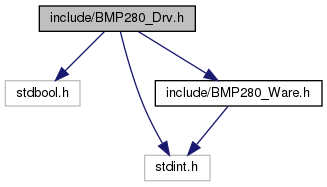
\includegraphics[width=318pt]{BMP280__Drv_8h__incl}
\end{center}
\end{figure}
This graph shows which files directly or indirectly include this file\+:\nopagebreak
\begin{figure}[H]
\begin{center}
\leavevmode
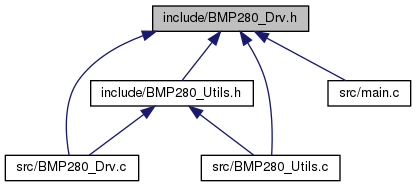
\includegraphics[width=350pt]{BMP280__Drv_8h__dep__incl}
\end{center}
\end{figure}
\subsection*{Data Structures}
\begin{DoxyCompactItemize}
\item 
struct \hyperlink{structBmp280Status}{Bmp280\+Status}
\begin{DoxyCompactList}\small\item\em indicate status of the bmp280 \end{DoxyCompactList}\item 
struct \hyperlink{structbmp280Sensor}{bmp280\+Sensor}
\begin{DoxyCompactList}\small\item\em data structure of a bmp280 \end{DoxyCompactList}\end{DoxyCompactItemize}
\subsection*{Typedefs}
\begin{DoxyCompactItemize}
\item 
\mbox{\Hypertarget{BMP280__Drv_8h_ab9e22f3267ce8af4053eb1189db84627}\label{BMP280__Drv_8h_ab9e22f3267ce8af4053eb1189db84627}} 
typedef struct \hyperlink{structbmp280Sensor}{bmp280\+Sensor} \hyperlink{BMP280__Drv_8h_ab9e22f3267ce8af4053eb1189db84627}{bmp280}
\begin{DoxyCompactList}\small\item\em data structure of a bmp280 \end{DoxyCompactList}\end{DoxyCompactItemize}
\subsection*{Enumerations}
\begin{DoxyCompactItemize}
\item 
\mbox{\Hypertarget{BMP280__Drv_8h_ab4295e33e8c981aef15803030d176782}\label{BMP280__Drv_8h_ab4295e33e8c981aef15803030d176782}} 
enum \hyperlink{BMP280__Drv_8h_ab4295e33e8c981aef15803030d176782}{Bmp280\+Com\+Protocol} \{ {\bfseries S\+PI}, 
{\bfseries I2C}
 \}\begin{DoxyCompactList}\small\item\em enum of all the sensors\textquotesingle{} settings and error code \end{DoxyCompactList}
\item 
\mbox{\Hypertarget{BMP280__Drv_8h_a4a0fcacff61a12b6888fc060fc2baddb}\label{BMP280__Drv_8h_a4a0fcacff61a12b6888fc060fc2baddb}} 
enum \hyperlink{BMP280__Drv_8h_a4a0fcacff61a12b6888fc060fc2baddb}{Bmp280\+Measure\+Settings} \{ \newline
{\bfseries Hand\+Low} = 0, 
{\bfseries Hand\+Dynamic}, 
{\bfseries Weather\+Stat}, 
{\bfseries Elev\+Detec}, 
\newline
{\bfseries Drop\+Detec}, 
{\bfseries Indoor\+Nav}, 
{\bfseries Custom}
 \}\begin{DoxyCompactList}\small\item\em predefined settings given by datasheet \end{DoxyCompactList}
\item 
\mbox{\Hypertarget{BMP280__Drv_8h_abd075292d5e9d310574c56eb88e4e05d}\label{BMP280__Drv_8h_abd075292d5e9d310574c56eb88e4e05d}} 
enum \hyperlink{BMP280__Drv_8h_abd075292d5e9d310574c56eb88e4e05d}{Bmp280\+Oper\+Mode} \{ {\bfseries Uninitialized\+\_\+mode} = -\/1, 
{\bfseries Sleep}, 
{\bfseries Forced}, 
{\bfseries Normal}
 \}\begin{DoxyCompactList}\small\item\em power mode of the bmp280 sensor \end{DoxyCompactList}
\item 
\mbox{\Hypertarget{BMP280__Drv_8h_ad55d98fff432892b33bf3f478e1bfbb2}\label{BMP280__Drv_8h_ad55d98fff432892b33bf3f478e1bfbb2}} 
enum \hyperlink{BMP280__Drv_8h_ad55d98fff432892b33bf3f478e1bfbb2}{Bmp280\+Sampl\+Settings} \{ \newline
{\bfseries Uninitialized} = -\/1, 
{\bfseries Ultra\+Low}, 
{\bfseries Low}, 
{\bfseries Standard}, 
\newline
{\bfseries Ultra\+High}
 \}\begin{DoxyCompactList}\small\item\em name of predefined oversampling settings \end{DoxyCompactList}
\item 
\mbox{\Hypertarget{BMP280__Drv_8h_ab15230ba27bac36bf1ba14a32fcd4d04}\label{BMP280__Drv_8h_ab15230ba27bac36bf1ba14a32fcd4d04}} 
enum \hyperlink{BMP280__Drv_8h_ab15230ba27bac36bf1ba14a32fcd4d04}{Bmp280\+Coeff} \{ \newline
{\bfseries Uninitialized\+\_\+coeff} = -\/1, 
{\bfseries x0}, 
{\bfseries x1}, 
{\bfseries x2}, 
\newline
{\bfseries x4}, 
{\bfseries x8}, 
{\bfseries x16}
 \}\begin{DoxyCompactList}\small\item\em used for I\+IR filter, temp and pressure oversampling coefficience \end{DoxyCompactList}
\item 
enum \hyperlink{BMP280__Drv_8h_a726300a3932e443ece00fcc5c4f3ca7c}{Bmp280\+Err\+Code} \{ \newline
\hyperlink{BMP280__Drv_8h_a726300a3932e443ece00fcc5c4f3ca7cab8516ccf594649942dde7e22723cdfa9}{E\+R\+R\+\_\+\+N\+O\+\_\+\+E\+RR}, 
{\bfseries E\+R\+R\+\_\+\+P\+O\+R\+T\+\_\+\+N\+O\+T\+\_\+\+O\+P\+EN}, 
{\bfseries E\+R\+R\+\_\+\+S\+E\+T\+T\+I\+N\+G\+\_\+\+U\+N\+I\+T\+I\+A\+L\+I\+Z\+ED}, 
{\bfseries E\+R\+R\+\_\+\+S\+E\+T\+T\+I\+N\+G\+\_\+\+U\+N\+R\+E\+C\+O\+G\+N\+I\+Z\+ED}, 
\newline
\hyperlink{BMP280__Drv_8h_a726300a3932e443ece00fcc5c4f3ca7ca0ae301ef0d5deb16d7b8521d21c6bf18}{E\+R\+R\+\_\+\+S\+E\+N\+S\+O\+R\+\_\+\+U\+N\+I\+T\+I\+A\+L\+I\+Z\+ED}
 \}\begin{DoxyCompactList}\small\item\em error code for the bmp280 \end{DoxyCompactList}
\end{DoxyCompactItemize}
\subsection*{Functions}
\begin{DoxyCompactItemize}
\item 
\hyperlink{BMP280__Drv_8h_a726300a3932e443ece00fcc5c4f3ca7c}{Bmp280\+Err\+Code} \hyperlink{BMP280__Drv_8h_a688a1cfffa854195e06f133867897012}{bmp280\+\_\+create\+\_\+predefined\+\_\+settings} (\hyperlink{BMP280__Drv_8h_ab9e22f3267ce8af4053eb1189db84627}{bmp280} $\ast$sensor, const \hyperlink{BMP280__Drv_8h_a4a0fcacff61a12b6888fc060fc2baddb}{Bmp280\+Measure\+Settings} settings)
\begin{DoxyCompactList}\small\item\em initialize the bmp280 with predefined value in the datasheet \end{DoxyCompactList}\item 
\mbox{\Hypertarget{BMP280__Drv_8h_a96a0359c3e21d58fdda67c171c864f5c}\label{BMP280__Drv_8h_a96a0359c3e21d58fdda67c171c864f5c}} 
\hyperlink{BMP280__Drv_8h_a726300a3932e443ece00fcc5c4f3ca7c}{Bmp280\+Err\+Code} \hyperlink{BMP280__Drv_8h_a96a0359c3e21d58fdda67c171c864f5c}{bmp280\+\_\+init} (\hyperlink{BMP280__Drv_8h_ab9e22f3267ce8af4053eb1189db84627}{bmp280} $\ast$sensor, const \hyperlink{BMP280__Drv_8h_ab4295e33e8c981aef15803030d176782}{Bmp280\+Com\+Protocol} protocol, const uint8\+\_\+t address)
\begin{DoxyCompactList}\small\item\em check settings, set the bmp280 address and desired communication protocols \end{DoxyCompactList}\item 
\mbox{\Hypertarget{BMP280__Drv_8h_a11548c71a21d35f741ec3a93911b8dd3}\label{BMP280__Drv_8h_a11548c71a21d35f741ec3a93911b8dd3}} 
\hyperlink{BMP280__Drv_8h_a726300a3932e443ece00fcc5c4f3ca7c}{Bmp280\+Err\+Code} \hyperlink{BMP280__Drv_8h_a11548c71a21d35f741ec3a93911b8dd3}{bmp280\+\_\+open} (\hyperlink{BMP280__Drv_8h_ab9e22f3267ce8af4053eb1189db84627}{bmp280} $\ast$sensor)
\begin{DoxyCompactList}\small\item\em prepare the i2c/spi port for communications \end{DoxyCompactList}\item 
\mbox{\Hypertarget{BMP280__Drv_8h_ab82a00168f6bf168223cda858f8d7357}\label{BMP280__Drv_8h_ab82a00168f6bf168223cda858f8d7357}} 
\hyperlink{BMP280__Drv_8h_a726300a3932e443ece00fcc5c4f3ca7c}{Bmp280\+Err\+Code} \hyperlink{BMP280__Drv_8h_ab82a00168f6bf168223cda858f8d7357}{bmp280\+\_\+close} (\hyperlink{BMP280__Drv_8h_ab9e22f3267ce8af4053eb1189db84627}{bmp280} $\ast$sensor)
\begin{DoxyCompactList}\small\item\em close the ports \end{DoxyCompactList}\item 
\mbox{\Hypertarget{BMP280__Drv_8h_aacbc533b2f3eebfd424f5ac45d5352d4}\label{BMP280__Drv_8h_aacbc533b2f3eebfd424f5ac45d5352d4}} 
\hyperlink{BMP280__Drv_8h_a726300a3932e443ece00fcc5c4f3ca7c}{Bmp280\+Err\+Code} \hyperlink{BMP280__Drv_8h_aacbc533b2f3eebfd424f5ac45d5352d4}{bmp280\+\_\+update\+\_\+setting} (\hyperlink{BMP280__Drv_8h_ab9e22f3267ce8af4053eb1189db84627}{bmp280} $\ast$sensor)
\begin{DoxyCompactList}\small\item\em used to write setting sin the bmp280 struct to the control and config register of the bmp280 \end{DoxyCompactList}\item 
\mbox{\Hypertarget{BMP280__Drv_8h_ab05eaeb6f32d42bb090af62454d84a49}\label{BMP280__Drv_8h_ab05eaeb6f32d42bb090af62454d84a49}} 
\hyperlink{BMP280__Drv_8h_a726300a3932e443ece00fcc5c4f3ca7c}{Bmp280\+Err\+Code} \hyperlink{BMP280__Drv_8h_ab05eaeb6f32d42bb090af62454d84a49}{bmp280\+\_\+get\+\_\+id} (\hyperlink{BMP280__Drv_8h_ab9e22f3267ce8af4053eb1189db84627}{bmp280} $\ast$sensor, uint8\+\_\+t $\ast$ID)
\begin{DoxyCompactList}\small\item\em get bmp280 sensor ID, should 0x58 or 88 in decimal \end{DoxyCompactList}\item 
\mbox{\Hypertarget{BMP280__Drv_8h_acdbe6877699dee241e19b12fcc4e28dc}\label{BMP280__Drv_8h_acdbe6877699dee241e19b12fcc4e28dc}} 
\hyperlink{BMP280__Drv_8h_a726300a3932e443ece00fcc5c4f3ca7c}{Bmp280\+Err\+Code} {\bfseries bmp280\+\_\+get\+\_\+temp} (\hyperlink{BMP280__Drv_8h_ab9e22f3267ce8af4053eb1189db84627}{bmp280} $\ast$sensor, float $\ast$temperature)
\item 
\mbox{\Hypertarget{BMP280__Drv_8h_ae30a5d4fbde1e89be3cf1185a527887a}\label{BMP280__Drv_8h_ae30a5d4fbde1e89be3cf1185a527887a}} 
\hyperlink{BMP280__Drv_8h_a726300a3932e443ece00fcc5c4f3ca7c}{Bmp280\+Err\+Code} {\bfseries bmp280\+\_\+get\+\_\+press} (\hyperlink{BMP280__Drv_8h_ab9e22f3267ce8af4053eb1189db84627}{bmp280} $\ast$sensor, float $\ast$pressure)
\item 
\hyperlink{BMP280__Drv_8h_a726300a3932e443ece00fcc5c4f3ca7c}{Bmp280\+Err\+Code} \hyperlink{BMP280__Drv_8h_aa851f088396c0bc027255aaff4303e5b}{bmp280\+\_\+get\+\_\+temp\+\_\+press} (\hyperlink{BMP280__Drv_8h_ab9e22f3267ce8af4053eb1189db84627}{bmp280} $\ast$sensor, float $\ast$temperatureC, float $\ast$press\+Pa, \hyperlink{structBmp280CalibParam}{Bmp280\+Calib\+Param} calib\+Param)
\begin{DoxyCompactList}\small\item\em used to read compensated temperature and pressure \end{DoxyCompactList}\item 
\mbox{\Hypertarget{BMP280__Drv_8h_a6e3c8eaf93ed264d21487663bb5badd4}\label{BMP280__Drv_8h_a6e3c8eaf93ed264d21487663bb5badd4}} 
\hyperlink{BMP280__Drv_8h_a726300a3932e443ece00fcc5c4f3ca7c}{Bmp280\+Err\+Code} \hyperlink{BMP280__Drv_8h_a6e3c8eaf93ed264d21487663bb5badd4}{bmp280\+\_\+reset} (\hyperlink{BMP280__Drv_8h_ab9e22f3267ce8af4053eb1189db84627}{bmp280} $\ast$sensor)
\begin{DoxyCompactList}\small\item\em perform power reset on the bmp280 There is a 5ms seconds delay to allow the bmp280 to properly wake up \end{DoxyCompactList}\item 
\mbox{\Hypertarget{BMP280__Drv_8h_a8d6eaf2deab89137c393ac5006214cc2}\label{BMP280__Drv_8h_a8d6eaf2deab89137c393ac5006214cc2}} 
\hyperlink{BMP280__Drv_8h_a726300a3932e443ece00fcc5c4f3ca7c}{Bmp280\+Err\+Code} \hyperlink{BMP280__Drv_8h_a8d6eaf2deab89137c393ac5006214cc2}{bmp280\+\_\+get\+\_\+ctr\+\_\+meas} (\hyperlink{BMP280__Drv_8h_ab9e22f3267ce8af4053eb1189db84627}{bmp280} $\ast$sensor, uint8\+\_\+t $\ast$ctrl\+Meas\+Rtr)
\begin{DoxyCompactList}\small\item\em read data from control register \end{DoxyCompactList}\item 
\mbox{\Hypertarget{BMP280__Drv_8h_ab2f0b73d65e47addcb3c3e40998de5be}\label{BMP280__Drv_8h_ab2f0b73d65e47addcb3c3e40998de5be}} 
\hyperlink{BMP280__Drv_8h_a726300a3932e443ece00fcc5c4f3ca7c}{Bmp280\+Err\+Code} \hyperlink{BMP280__Drv_8h_ab2f0b73d65e47addcb3c3e40998de5be}{bmp280\+\_\+get\+\_\+config} (\hyperlink{BMP280__Drv_8h_ab9e22f3267ce8af4053eb1189db84627}{bmp280} $\ast$sensor, uint8\+\_\+t $\ast$config\+Return)
\begin{DoxyCompactList}\small\item\em read data from config register \end{DoxyCompactList}\item 
\mbox{\Hypertarget{BMP280__Drv_8h_aa6a7975dfb6b2f86ad4a63ce5c32be3e}\label{BMP280__Drv_8h_aa6a7975dfb6b2f86ad4a63ce5c32be3e}} 
\hyperlink{BMP280__Drv_8h_a726300a3932e443ece00fcc5c4f3ca7c}{Bmp280\+Err\+Code} \hyperlink{BMP280__Drv_8h_aa6a7975dfb6b2f86ad4a63ce5c32be3e}{bmp280\+\_\+get\+\_\+calibration\+\_\+data} (\hyperlink{BMP280__Drv_8h_ab9e22f3267ce8af4053eb1189db84627}{bmp280} $\ast$sensor, \hyperlink{structBmp280CalibParam}{Bmp280\+Calib\+Param} $\ast$calib\+Param)
\begin{DoxyCompactList}\small\item\em used to read factory calibration data from the bmp280 \end{DoxyCompactList}\item 
\mbox{\Hypertarget{BMP280__Drv_8h_aae4895c0b12a1ced41bbfa71ee5b074c}\label{BMP280__Drv_8h_aae4895c0b12a1ced41bbfa71ee5b074c}} 
\hyperlink{BMP280__Drv_8h_a726300a3932e443ece00fcc5c4f3ca7c}{Bmp280\+Err\+Code} \hyperlink{BMP280__Drv_8h_aae4895c0b12a1ced41bbfa71ee5b074c}{bmp280\+\_\+get\+\_\+status} (\hyperlink{BMP280__Drv_8h_ab9e22f3267ce8af4053eb1189db84627}{bmp280} $\ast$sensor)
\begin{DoxyCompactList}\small\item\em read bmp280 status and change last known status of the sensor \end{DoxyCompactList}\item 
\hyperlink{BMP280__Drv_8h_a726300a3932e443ece00fcc5c4f3ca7c}{Bmp280\+Err\+Code} \hyperlink{BMP280__Drv_8h_a61a00b8689733032a3148c7a37990be2}{bmp280\+\_\+create\+\_\+custom\+\_\+setting} (\hyperlink{BMP280__Drv_8h_ab9e22f3267ce8af4053eb1189db84627}{bmp280} $\ast$sensor, const \hyperlink{BMP280__Drv_8h_ab15230ba27bac36bf1ba14a32fcd4d04}{Bmp280\+Coeff} temp\+Samp, const \hyperlink{BMP280__Drv_8h_ab15230ba27bac36bf1ba14a32fcd4d04}{Bmp280\+Coeff} pres\+Samp, const \hyperlink{BMP280__Drv_8h_ab15230ba27bac36bf1ba14a32fcd4d04}{Bmp280\+Coeff} iir\+Filter, const \hyperlink{BMP280__Drv_8h_ad55d98fff432892b33bf3f478e1bfbb2}{Bmp280\+Sampl\+Settings} sampl\+Set, const \hyperlink{BMP280__Drv_8h_abd075292d5e9d310574c56eb88e4e05d}{Bmp280\+Oper\+Mode} mode, const float standby\+Time)
\begin{DoxyCompactList}\small\item\em initialize the bmp280 struct with options from user \end{DoxyCompactList}\end{DoxyCompactItemize}


\subsection{Detailed Description}
contain data structures for B\+M\+P280 

\begin{DoxyAuthor}{Author}
Khoi Trinh 
\end{DoxyAuthor}
\begin{DoxyDate}{Date}
2018-\/08-\/25 
\end{DoxyDate}


\subsection{Enumeration Type Documentation}
\mbox{\Hypertarget{BMP280__Drv_8h_a726300a3932e443ece00fcc5c4f3ca7c}\label{BMP280__Drv_8h_a726300a3932e443ece00fcc5c4f3ca7c}} 
\index{B\+M\+P280\+\_\+\+Drv.\+h@{B\+M\+P280\+\_\+\+Drv.\+h}!Bmp280\+Err\+Code@{Bmp280\+Err\+Code}}
\index{Bmp280\+Err\+Code@{Bmp280\+Err\+Code}!B\+M\+P280\+\_\+\+Drv.\+h@{B\+M\+P280\+\_\+\+Drv.\+h}}
\subsubsection{\texorpdfstring{Bmp280\+Err\+Code}{Bmp280ErrCode}}
{\footnotesize\ttfamily enum \hyperlink{BMP280__Drv_8h_a726300a3932e443ece00fcc5c4f3ca7c}{Bmp280\+Err\+Code}}



error code for the bmp280 

\begin{DoxyEnumFields}{Enumerator}
\raisebox{\heightof{T}}[0pt][0pt]{\index{E\+R\+R\+\_\+\+N\+O\+\_\+\+E\+RR@{E\+R\+R\+\_\+\+N\+O\+\_\+\+E\+RR}!B\+M\+P280\+\_\+\+Drv.\+h@{B\+M\+P280\+\_\+\+Drv.\+h}}\index{B\+M\+P280\+\_\+\+Drv.\+h@{B\+M\+P280\+\_\+\+Drv.\+h}!E\+R\+R\+\_\+\+N\+O\+\_\+\+E\+RR@{E\+R\+R\+\_\+\+N\+O\+\_\+\+E\+RR}}}\mbox{\Hypertarget{BMP280__Drv_8h_a726300a3932e443ece00fcc5c4f3ca7cab8516ccf594649942dde7e22723cdfa9}\label{BMP280__Drv_8h_a726300a3932e443ece00fcc5c4f3ca7cab8516ccf594649942dde7e22723cdfa9}} 
E\+R\+R\+\_\+\+N\+O\+\_\+\+E\+RR&report that there is no error \\
\hline

\raisebox{\heightof{T}}[0pt][0pt]{\index{E\+R\+R\+\_\+\+S\+E\+N\+S\+O\+R\+\_\+\+U\+N\+I\+T\+I\+A\+L\+I\+Z\+ED@{E\+R\+R\+\_\+\+S\+E\+N\+S\+O\+R\+\_\+\+U\+N\+I\+T\+I\+A\+L\+I\+Z\+ED}!B\+M\+P280\+\_\+\+Drv.\+h@{B\+M\+P280\+\_\+\+Drv.\+h}}\index{B\+M\+P280\+\_\+\+Drv.\+h@{B\+M\+P280\+\_\+\+Drv.\+h}!E\+R\+R\+\_\+\+S\+E\+N\+S\+O\+R\+\_\+\+U\+N\+I\+T\+I\+A\+L\+I\+Z\+ED@{E\+R\+R\+\_\+\+S\+E\+N\+S\+O\+R\+\_\+\+U\+N\+I\+T\+I\+A\+L\+I\+Z\+ED}}}\mbox{\Hypertarget{BMP280__Drv_8h_a726300a3932e443ece00fcc5c4f3ca7ca0ae301ef0d5deb16d7b8521d21c6bf18}\label{BMP280__Drv_8h_a726300a3932e443ece00fcc5c4f3ca7ca0ae301ef0d5deb16d7b8521d21c6bf18}} 
E\+R\+R\+\_\+\+S\+E\+N\+S\+O\+R\+\_\+\+U\+N\+I\+T\+I\+A\+L\+I\+Z\+ED&indicate that bmp280 struct is not valid \\
\hline

\end{DoxyEnumFields}


\subsection{Function Documentation}
\mbox{\Hypertarget{BMP280__Drv_8h_a61a00b8689733032a3148c7a37990be2}\label{BMP280__Drv_8h_a61a00b8689733032a3148c7a37990be2}} 
\index{B\+M\+P280\+\_\+\+Drv.\+h@{B\+M\+P280\+\_\+\+Drv.\+h}!bmp280\+\_\+create\+\_\+custom\+\_\+setting@{bmp280\+\_\+create\+\_\+custom\+\_\+setting}}
\index{bmp280\+\_\+create\+\_\+custom\+\_\+setting@{bmp280\+\_\+create\+\_\+custom\+\_\+setting}!B\+M\+P280\+\_\+\+Drv.\+h@{B\+M\+P280\+\_\+\+Drv.\+h}}
\subsubsection{\texorpdfstring{bmp280\+\_\+create\+\_\+custom\+\_\+setting()}{bmp280\_create\_custom\_setting()}}
{\footnotesize\ttfamily \hyperlink{BMP280__Drv_8h_a726300a3932e443ece00fcc5c4f3ca7c}{Bmp280\+Err\+Code} bmp280\+\_\+create\+\_\+custom\+\_\+setting (\begin{DoxyParamCaption}\item[{\hyperlink{BMP280__Drv_8h_ab9e22f3267ce8af4053eb1189db84627}{bmp280} $\ast$}]{sensor,  }\item[{const \hyperlink{BMP280__Drv_8h_ab15230ba27bac36bf1ba14a32fcd4d04}{Bmp280\+Coeff}}]{temp\+Samp,  }\item[{const \hyperlink{BMP280__Drv_8h_ab15230ba27bac36bf1ba14a32fcd4d04}{Bmp280\+Coeff}}]{pres\+Samp,  }\item[{const \hyperlink{BMP280__Drv_8h_ab15230ba27bac36bf1ba14a32fcd4d04}{Bmp280\+Coeff}}]{iir\+Filter,  }\item[{const \hyperlink{BMP280__Drv_8h_ad55d98fff432892b33bf3f478e1bfbb2}{Bmp280\+Sampl\+Settings}}]{sampl\+Set,  }\item[{const \hyperlink{BMP280__Drv_8h_abd075292d5e9d310574c56eb88e4e05d}{Bmp280\+Oper\+Mode}}]{mode,  }\item[{const float}]{standby\+Time }\end{DoxyParamCaption})}



initialize the bmp280 struct with options from user 

\begin{DoxyReturn}{Returns}
no error or user settings violated some rules 
\end{DoxyReturn}
\mbox{\Hypertarget{BMP280__Drv_8h_a688a1cfffa854195e06f133867897012}\label{BMP280__Drv_8h_a688a1cfffa854195e06f133867897012}} 
\index{B\+M\+P280\+\_\+\+Drv.\+h@{B\+M\+P280\+\_\+\+Drv.\+h}!bmp280\+\_\+create\+\_\+predefined\+\_\+settings@{bmp280\+\_\+create\+\_\+predefined\+\_\+settings}}
\index{bmp280\+\_\+create\+\_\+predefined\+\_\+settings@{bmp280\+\_\+create\+\_\+predefined\+\_\+settings}!B\+M\+P280\+\_\+\+Drv.\+h@{B\+M\+P280\+\_\+\+Drv.\+h}}
\subsubsection{\texorpdfstring{bmp280\+\_\+create\+\_\+predefined\+\_\+settings()}{bmp280\_create\_predefined\_settings()}}
{\footnotesize\ttfamily \hyperlink{BMP280__Drv_8h_a726300a3932e443ece00fcc5c4f3ca7c}{Bmp280\+Err\+Code} bmp280\+\_\+create\+\_\+predefined\+\_\+settings (\begin{DoxyParamCaption}\item[{\hyperlink{BMP280__Drv_8h_ab9e22f3267ce8af4053eb1189db84627}{bmp280} $\ast$}]{sensor,  }\item[{const \hyperlink{BMP280__Drv_8h_a4a0fcacff61a12b6888fc060fc2baddb}{Bmp280\+Measure\+Settings}}]{settings }\end{DoxyParamCaption})}



initialize the bmp280 with predefined value in the datasheet 

\begin{DoxyReturn}{Returns}
no error or user settings violated some rules 
\end{DoxyReturn}
\mbox{\Hypertarget{BMP280__Drv_8h_aa851f088396c0bc027255aaff4303e5b}\label{BMP280__Drv_8h_aa851f088396c0bc027255aaff4303e5b}} 
\index{B\+M\+P280\+\_\+\+Drv.\+h@{B\+M\+P280\+\_\+\+Drv.\+h}!bmp280\+\_\+get\+\_\+temp\+\_\+press@{bmp280\+\_\+get\+\_\+temp\+\_\+press}}
\index{bmp280\+\_\+get\+\_\+temp\+\_\+press@{bmp280\+\_\+get\+\_\+temp\+\_\+press}!B\+M\+P280\+\_\+\+Drv.\+h@{B\+M\+P280\+\_\+\+Drv.\+h}}
\subsubsection{\texorpdfstring{bmp280\+\_\+get\+\_\+temp\+\_\+press()}{bmp280\_get\_temp\_press()}}
{\footnotesize\ttfamily \hyperlink{BMP280__Drv_8h_a726300a3932e443ece00fcc5c4f3ca7c}{Bmp280\+Err\+Code} bmp280\+\_\+get\+\_\+temp\+\_\+press (\begin{DoxyParamCaption}\item[{\hyperlink{BMP280__Drv_8h_ab9e22f3267ce8af4053eb1189db84627}{bmp280} $\ast$}]{sensor,  }\item[{float $\ast$}]{temperatureC,  }\item[{float $\ast$}]{press\+Pa,  }\item[{\hyperlink{structBmp280CalibParam}{Bmp280\+Calib\+Param}}]{calib\+Param }\end{DoxyParamCaption})}



used to read compensated temperature and pressure 


\begin{DoxyParams}{Parameters}
{\em temperatureC} & return temperature \\
\hline
{\em press\+Pa} & return pressure \\
\hline
{\em calib\+Param} & calibration data obtained beforehand \\
\hline
\end{DoxyParams}

\hypertarget{BMP280__Utils_8h}{}\section{include/\+B\+M\+P280\+\_\+\+Utils.h File Reference}
\label{BMP280__Utils_8h}\index{include/\+B\+M\+P280\+\_\+\+Utils.\+h@{include/\+B\+M\+P280\+\_\+\+Utils.\+h}}


headers to B\+M\+P280 utils functions  


{\ttfamily \#include $<$stdint.\+h$>$}\newline
{\ttfamily \#include \char`\"{}include/\+B\+M\+P280\+\_\+\+Drv.\+h\char`\"{}}\newline
Include dependency graph for B\+M\+P280\+\_\+\+Utils.\+h\+:\nopagebreak
\begin{figure}[H]
\begin{center}
\leavevmode
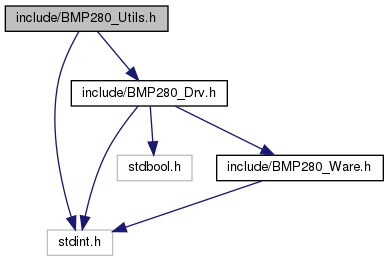
\includegraphics[width=350pt]{BMP280__Utils_8h__incl}
\end{center}
\end{figure}
This graph shows which files directly or indirectly include this file\+:\nopagebreak
\begin{figure}[H]
\begin{center}
\leavevmode
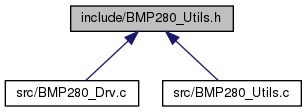
\includegraphics[width=302pt]{BMP280__Utils_8h__dep__incl}
\end{center}
\end{figure}
\subsection*{Macros}
\begin{DoxyCompactItemize}
\item 
\#define {\bfseries B\+M\+P280\+\_\+\+T\+R\+Y\+\_\+\+F\+U\+NC}(func\+To\+Execute)
\end{DoxyCompactItemize}
\subsection*{Functions}
\begin{DoxyCompactItemize}
\item 
\mbox{\Hypertarget{BMP280__Utils_8h_a651c00a3684abdf07d2573d92fe45b63}\label{BMP280__Utils_8h_a651c00a3684abdf07d2573d92fe45b63}} 
\hyperlink{BMP280__Drv_8h_a726300a3932e443ece00fcc5c4f3ca7c}{Bmp280\+Err\+Code} \hyperlink{BMP280__Utils_8h_a651c00a3684abdf07d2573d92fe45b63}{bmp280\+\_\+make\+\_\+ctrl\+\_\+byte} (\hyperlink{BMP280__Drv_8h_ab9e22f3267ce8af4053eb1189db84627}{bmp280} $\ast$sensor, uint8\+\_\+t $\ast$control\+Byte)
\begin{DoxyCompactList}\small\item\em create a byte corresponding to user option to be sent to the control register on the B\+M\+P280 \end{DoxyCompactList}\item 
\mbox{\Hypertarget{BMP280__Utils_8h_a4045241afbda61ce8354f7cbb25539bc}\label{BMP280__Utils_8h_a4045241afbda61ce8354f7cbb25539bc}} 
uint8\+\_\+t \hyperlink{BMP280__Utils_8h_a4045241afbda61ce8354f7cbb25539bc}{bmp280\+\_\+make\+\_\+cfg\+\_\+byte} (\hyperlink{BMP280__Drv_8h_ab9e22f3267ce8af4053eb1189db84627}{bmp280} $\ast$sensor, uint8\+\_\+t $\ast$return\+Byte)
\begin{DoxyCompactList}\small\item\em create a byte corresponding to user option to be sent to the config register on the B\+M\+P280 \end{DoxyCompactList}\item 
\mbox{\Hypertarget{BMP280__Utils_8h_a36f6ebcb6c407ee4e48a741bc77b580e}\label{BMP280__Utils_8h_a36f6ebcb6c407ee4e48a741bc77b580e}} 
\hyperlink{BMP280__Drv_8h_a726300a3932e443ece00fcc5c4f3ca7c}{Bmp280\+Err\+Code} \hyperlink{BMP280__Utils_8h_a36f6ebcb6c407ee4e48a741bc77b580e}{bmp280\+\_\+check\+\_\+setting} (\hyperlink{BMP280__Drv_8h_ab9e22f3267ce8af4053eb1189db84627}{bmp280} $\ast$sensor)
\begin{DoxyCompactList}\small\item\em check user settings to make sure they are among the supported options \end{DoxyCompactList}\item 
\mbox{\Hypertarget{BMP280__Utils_8h_a17288e03b956c789447940fb2ea10c88}\label{BMP280__Utils_8h_a17288e03b956c789447940fb2ea10c88}} 
\hyperlink{BMP280__Drv_8h_a726300a3932e443ece00fcc5c4f3ca7c}{Bmp280\+Err\+Code} \hyperlink{BMP280__Utils_8h_a17288e03b956c789447940fb2ea10c88}{bmp280\+\_\+port\+\_\+check} (\hyperlink{BMP280__Drv_8h_ab9e22f3267ce8af4053eb1189db84627}{bmp280} $\ast$sensor)
\begin{DoxyCompactList}\small\item\em port check that are run before data communication \end{DoxyCompactList}\item 
\mbox{\Hypertarget{BMP280__Utils_8h_a98f791b4ff6fcabbe466bbfabf0cb8f5}\label{BMP280__Utils_8h_a98f791b4ff6fcabbe466bbfabf0cb8f5}} 
\hyperlink{BMP280__Drv_8h_a726300a3932e443ece00fcc5c4f3ca7c}{Bmp280\+Err\+Code} \hyperlink{BMP280__Utils_8h_a98f791b4ff6fcabbe466bbfabf0cb8f5}{bmp280\+\_\+port\+\_\+prep} (\hyperlink{BMP280__Drv_8h_ab9e22f3267ce8af4053eb1189db84627}{bmp280} $\ast$sensor)
\begin{DoxyCompactList}\small\item\em things to run to prep the i2c/spi port for communication \end{DoxyCompactList}\item 
\mbox{\Hypertarget{BMP280__Utils_8h_a0b70b2b744d683d210f703a83cac2e6c}\label{BMP280__Utils_8h_a0b70b2b744d683d210f703a83cac2e6c}} 
\hyperlink{BMP280__Drv_8h_a726300a3932e443ece00fcc5c4f3ca7c}{Bmp280\+Err\+Code} \hyperlink{BMP280__Utils_8h_a0b70b2b744d683d210f703a83cac2e6c}{bmp280\+\_\+get\+\_\+register} (\hyperlink{BMP280__Drv_8h_ab9e22f3267ce8af4053eb1189db84627}{bmp280} $\ast$sensor, const uint8\+\_\+t start\+Addr, uint8\+\_\+t $\ast$reg\+Data, const uint8\+\_\+t total\+Register)
\begin{DoxyCompactList}\small\item\em protocol agnostic function to get data from one or multiple register \end{DoxyCompactList}\item 
\mbox{\Hypertarget{BMP280__Utils_8h_a32b99e7c569d0b4e0aa6829994041171}\label{BMP280__Utils_8h_a32b99e7c569d0b4e0aa6829994041171}} 
\hyperlink{BMP280__Drv_8h_a726300a3932e443ece00fcc5c4f3ca7c}{Bmp280\+Err\+Code} \hyperlink{BMP280__Utils_8h_a32b99e7c569d0b4e0aa6829994041171}{bmp280\+\_\+write\+\_\+register} (\hyperlink{BMP280__Drv_8h_ab9e22f3267ce8af4053eb1189db84627}{bmp280} $\ast$sensor, const uint8\+\_\+t $\ast$register\+List, const uint8\+\_\+t total\+Register, const uint8\+\_\+t $\ast$register\+Data\+List)
\begin{DoxyCompactList}\small\item\em protocol agnostic function to write data to one or multiple register \end{DoxyCompactList}\item 
\mbox{\Hypertarget{BMP280__Utils_8h_a063d98e3e3b84c4c2816ff82e4c2aacd}\label{BMP280__Utils_8h_a063d98e3e3b84c4c2816ff82e4c2aacd}} 
\hyperlink{BMP280__Drv_8h_a726300a3932e443ece00fcc5c4f3ca7c}{Bmp280\+Err\+Code} \hyperlink{BMP280__Utils_8h_a063d98e3e3b84c4c2816ff82e4c2aacd}{bmp280\+\_\+open\+\_\+i2c\+\_\+spi} (\hyperlink{BMP280__Drv_8h_ab9e22f3267ce8af4053eb1189db84627}{bmp280} $\ast$sensor)
\begin{DoxyCompactList}\small\item\em open spi or i2c communications \end{DoxyCompactList}\item 
\mbox{\Hypertarget{BMP280__Utils_8h_a3475b11b628b6248e6848694d4450450}\label{BMP280__Utils_8h_a3475b11b628b6248e6848694d4450450}} 
\hyperlink{BMP280__Drv_8h_a726300a3932e443ece00fcc5c4f3ca7c}{Bmp280\+Err\+Code} \hyperlink{BMP280__Utils_8h_a3475b11b628b6248e6848694d4450450}{bmp280\+\_\+close\+\_\+i2c\+\_\+spi} (\hyperlink{BMP280__Drv_8h_ab9e22f3267ce8af4053eb1189db84627}{bmp280} $\ast$sensor)
\begin{DoxyCompactList}\small\item\em close i2c or spi communications \end{DoxyCompactList}\end{DoxyCompactItemize}


\subsection{Detailed Description}
headers to B\+M\+P280 utils functions 

\begin{DoxyAuthor}{Author}
Khoi Trinh 
\end{DoxyAuthor}
\begin{DoxyDate}{Date}
2018-\/08-\/25 
\end{DoxyDate}


\subsection{Macro Definition Documentation}
\mbox{\Hypertarget{BMP280__Utils_8h_a7b2fb7f0fc42f84778d7a4fb1ed0cc37}\label{BMP280__Utils_8h_a7b2fb7f0fc42f84778d7a4fb1ed0cc37}} 
\index{B\+M\+P280\+\_\+\+Utils.\+h@{B\+M\+P280\+\_\+\+Utils.\+h}!B\+M\+P280\+\_\+\+T\+R\+Y\+\_\+\+F\+U\+NC@{B\+M\+P280\+\_\+\+T\+R\+Y\+\_\+\+F\+U\+NC}}
\index{B\+M\+P280\+\_\+\+T\+R\+Y\+\_\+\+F\+U\+NC@{B\+M\+P280\+\_\+\+T\+R\+Y\+\_\+\+F\+U\+NC}!B\+M\+P280\+\_\+\+Utils.\+h@{B\+M\+P280\+\_\+\+Utils.\+h}}
\subsubsection{\texorpdfstring{B\+M\+P280\+\_\+\+T\+R\+Y\+\_\+\+F\+U\+NC}{BMP280\_TRY\_FUNC}}
{\footnotesize\ttfamily \#define B\+M\+P280\+\_\+\+T\+R\+Y\+\_\+\+F\+U\+NC(\begin{DoxyParamCaption}\item[{}]{func\+To\+Execute }\end{DoxyParamCaption})}

{\bfseries Value\+:}
\begin{DoxyCode}
\textcolor{keywordflow}{do} \{                                             \(\backslash\)
    Bmp280ErrCode errCode;                         \(\backslash\)
    errCode = funcToExecute;                       \(\backslash\)
    if (errCode != \hyperlink{BMP280__Drv_8h_a726300a3932e443ece00fcc5c4f3ca7cab8516ccf594649942dde7e22723cdfa9}{ERR\_NO\_ERR}) \{ \textcolor{keywordflow}{return} errCode; \} \(\backslash\)
  \} \textcolor{keywordflow}{while} (0)
\end{DoxyCode}

\hypertarget{BMP280__Ware_8h}{}\section{include/\+B\+M\+P280\+\_\+\+Ware.h File Reference}
\label{BMP280__Ware_8h}\index{include/\+B\+M\+P280\+\_\+\+Ware.\+h@{include/\+B\+M\+P280\+\_\+\+Ware.\+h}}


Utils header that contain Bosch data structure for calibration data as well as bit positions of data.  


{\ttfamily \#include $<$stdint.\+h$>$}\newline
Include dependency graph for B\+M\+P280\+\_\+\+Ware.\+h\+:\nopagebreak
\begin{figure}[H]
\begin{center}
\leavevmode
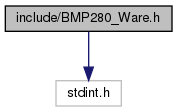
\includegraphics[width=205pt]{BMP280__Ware_8h__incl}
\end{center}
\end{figure}
This graph shows which files directly or indirectly include this file\+:\nopagebreak
\begin{figure}[H]
\begin{center}
\leavevmode
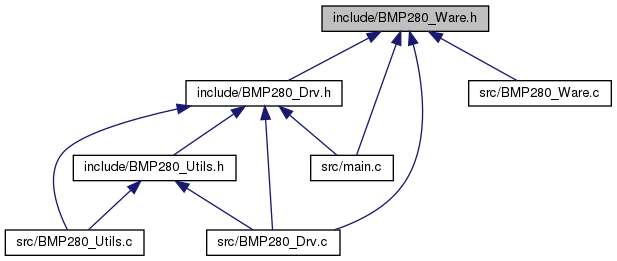
\includegraphics[width=350pt]{BMP280__Ware_8h__dep__incl}
\end{center}
\end{figure}
\subsection*{Data Structures}
\begin{DoxyCompactItemize}
\item 
struct \hyperlink{structBmp280CalibParam}{Bmp280\+Calib\+Param}
\begin{DoxyCompactList}\small\item\em calibration data struct \end{DoxyCompactList}\end{DoxyCompactItemize}
\subsection*{Calibration parameters\textquotesingle{} structure}
\label{_amgrp5165ce4c6c89fbfebaf2642db08fc6df}%
Copyright (C) 2017 -\/ 2018 Bosch Sensortec GmbH

Redistribution and use in source and binary forms, with or without modification, are permitted provided that the following conditions are met\+:

Redistributions of source code must retain the above copyright notice, this list of conditions and the following disclaimer.

Redistributions in binary form must reproduce the above copyright notice, this list of conditions and the following disclaimer in the documentation and/or other materials provided with the distribution.

Neither the name of the copyright holder nor the names of the contributors may be used to endorse or promote products derived from this software without specific prior written permission.

T\+H\+IS S\+O\+F\+T\+W\+A\+RE IS P\+R\+O\+V\+I\+D\+ED BY T\+HE C\+O\+P\+Y\+R\+I\+G\+HT H\+O\+L\+D\+E\+RS A\+ND C\+O\+N\+T\+R\+I\+B\+U\+T\+O\+RS \char`\"{}\+A\+S I\+S\char`\"{} A\+ND A\+NY E\+X\+P\+R\+E\+SS OR I\+M\+P\+L\+I\+ED W\+A\+R\+R\+A\+N\+T\+I\+ES, I\+N\+C\+L\+U\+D\+I\+NG, B\+UT N\+OT L\+I\+M\+I\+T\+ED TO, T\+HE I\+M\+P\+L\+I\+ED W\+A\+R\+R\+A\+N\+T\+I\+ES OF M\+E\+R\+C\+H\+A\+N\+T\+A\+B\+I\+L\+I\+TY A\+ND F\+I\+T\+N\+E\+SS F\+OR A P\+A\+R\+T\+I\+C\+U\+L\+AR P\+U\+R\+P\+O\+SE A\+RE D\+I\+S\+C\+L\+A\+I\+M\+ED. IN NO E\+V\+E\+NT S\+H\+A\+LL C\+O\+P\+Y\+R\+I\+G\+HT H\+O\+L\+D\+ER OR C\+O\+N\+T\+R\+I\+B\+U\+T\+O\+RS BE L\+I\+A\+B\+LE F\+OR A\+NY D\+I\+R\+E\+CT, I\+N\+D\+I\+R\+E\+CT, I\+N\+C\+I\+D\+E\+N\+T\+AL, S\+P\+E\+C\+I\+AL, E\+X\+E\+M\+P\+L\+A\+RY, OR C\+O\+N\+S\+E\+Q\+U\+E\+N\+T\+I\+AL D\+A\+M\+A\+G\+ES(I\+N\+C\+L\+U\+D\+I\+NG, B\+UT N\+OT L\+I\+M\+I\+T\+ED TO, P\+R\+O\+C\+U\+R\+E\+M\+E\+NT OF S\+U\+B\+S\+T\+I\+T\+U\+TE G\+O\+O\+DS OR S\+E\+R\+V\+I\+C\+ES; L\+O\+SS OF U\+SE, D\+A\+TA, OR P\+R\+O\+F\+I\+TS; OR B\+U\+S\+I\+N\+E\+SS I\+N\+T\+E\+R\+R\+U\+P\+T\+I\+ON) H\+O\+W\+E\+V\+ER C\+A\+U\+S\+ED A\+ND ON A\+NY T\+H\+E\+O\+RY OF L\+I\+A\+B\+I\+L\+I\+TY, W\+H\+E\+T\+H\+ER IN C\+O\+N\+T\+R\+A\+CT, S\+T\+R\+I\+CT L\+I\+A\+B\+I\+L\+I\+TY, OR T\+O\+RT (I\+N\+C\+L\+U\+D\+I\+NG N\+E\+G\+L\+I\+G\+E\+N\+CE OR O\+T\+H\+E\+R\+W\+I\+SE) A\+R\+I\+S\+I\+NG IN A\+NY W\+AY O\+UT OF T\+HE U\+SE OF T\+H\+IS S\+O\+F\+T\+W\+A\+RE, E\+V\+EN IF A\+D\+V\+I\+S\+ED OF T\+HE P\+O\+S\+S\+I\+B\+I\+L\+I\+TY OF S\+U\+CH D\+A\+M\+A\+GE

The information provided is believed to be accurate and reliable. The copyright holder assumes no responsibility for the consequences of use of such information nor for any infringement of patents or other rights of third parties which may result from its use. No license is granted by implication or otherwise under any patent or patent rights of the copyright holder. \begin{DoxyCompactItemize}
\item 
\mbox{\Hypertarget{BMP280__Ware_8h_ae65ac0ea31078810093f0099e025ae0e}\label{BMP280__Ware_8h_ae65ac0ea31078810093f0099e025ae0e}} 
\#define {\bfseries B\+M\+P280\+\_\+\+D\+I\+G\+\_\+\+T1\+\_\+\+L\+S\+B\+\_\+\+P\+OS}~U\+I\+N\+T8\+\_\+C(0)
\item 
\mbox{\Hypertarget{BMP280__Ware_8h_a5fa63c01c326f6ff3bab410e517ced7d}\label{BMP280__Ware_8h_a5fa63c01c326f6ff3bab410e517ced7d}} 
\#define {\bfseries B\+M\+P280\+\_\+\+D\+I\+G\+\_\+\+T1\+\_\+\+M\+S\+B\+\_\+\+P\+OS}~U\+I\+N\+T8\+\_\+C(1)
\item 
\mbox{\Hypertarget{BMP280__Ware_8h_ae1c6ff215996329427a319a4c48d694e}\label{BMP280__Ware_8h_ae1c6ff215996329427a319a4c48d694e}} 
\#define {\bfseries B\+M\+P280\+\_\+\+D\+I\+G\+\_\+\+T2\+\_\+\+L\+S\+B\+\_\+\+P\+OS}~U\+I\+N\+T8\+\_\+C(2)
\item 
\mbox{\Hypertarget{BMP280__Ware_8h_a7f24870e143963d87656a33fc4f0fbce}\label{BMP280__Ware_8h_a7f24870e143963d87656a33fc4f0fbce}} 
\#define {\bfseries B\+M\+P280\+\_\+\+D\+I\+G\+\_\+\+T2\+\_\+\+M\+S\+B\+\_\+\+P\+OS}~U\+I\+N\+T8\+\_\+C(3)
\item 
\mbox{\Hypertarget{BMP280__Ware_8h_a9df22f3020e2b53030be98b873cd5cb8}\label{BMP280__Ware_8h_a9df22f3020e2b53030be98b873cd5cb8}} 
\#define {\bfseries B\+M\+P280\+\_\+\+D\+I\+G\+\_\+\+T3\+\_\+\+L\+S\+B\+\_\+\+P\+OS}~U\+I\+N\+T8\+\_\+C(4)
\item 
\mbox{\Hypertarget{BMP280__Ware_8h_aee8c80b38d12d9cd18db0ef1c526dcfc}\label{BMP280__Ware_8h_aee8c80b38d12d9cd18db0ef1c526dcfc}} 
\#define {\bfseries B\+M\+P280\+\_\+\+D\+I\+G\+\_\+\+T3\+\_\+\+M\+S\+B\+\_\+\+P\+OS}~U\+I\+N\+T8\+\_\+C(5)
\item 
\mbox{\Hypertarget{BMP280__Ware_8h_afbf43c4330d2451d705066fbf403778d}\label{BMP280__Ware_8h_afbf43c4330d2451d705066fbf403778d}} 
\#define {\bfseries B\+M\+P280\+\_\+\+D\+I\+G\+\_\+\+P1\+\_\+\+L\+S\+B\+\_\+\+P\+OS}~U\+I\+N\+T8\+\_\+C(6)
\item 
\mbox{\Hypertarget{BMP280__Ware_8h_ad4f7f2bc990aceedc0b01a0170d19b21}\label{BMP280__Ware_8h_ad4f7f2bc990aceedc0b01a0170d19b21}} 
\#define {\bfseries B\+M\+P280\+\_\+\+D\+I\+G\+\_\+\+P1\+\_\+\+M\+S\+B\+\_\+\+P\+OS}~U\+I\+N\+T8\+\_\+C(7)
\item 
\mbox{\Hypertarget{BMP280__Ware_8h_ab421d3f027d0a9f132b215cff2148e9a}\label{BMP280__Ware_8h_ab421d3f027d0a9f132b215cff2148e9a}} 
\#define {\bfseries B\+M\+P280\+\_\+\+D\+I\+G\+\_\+\+P2\+\_\+\+L\+S\+B\+\_\+\+P\+OS}~U\+I\+N\+T8\+\_\+C(8)
\item 
\mbox{\Hypertarget{BMP280__Ware_8h_afec6f1ab60973c1c4380bd570b71b968}\label{BMP280__Ware_8h_afec6f1ab60973c1c4380bd570b71b968}} 
\#define {\bfseries B\+M\+P280\+\_\+\+D\+I\+G\+\_\+\+P2\+\_\+\+M\+S\+B\+\_\+\+P\+OS}~U\+I\+N\+T8\+\_\+C(9)
\item 
\mbox{\Hypertarget{BMP280__Ware_8h_aeb26dc721db438c236416175c6c528bb}\label{BMP280__Ware_8h_aeb26dc721db438c236416175c6c528bb}} 
\#define {\bfseries B\+M\+P280\+\_\+\+D\+I\+G\+\_\+\+P3\+\_\+\+L\+S\+B\+\_\+\+P\+OS}~U\+I\+N\+T8\+\_\+C(10)
\item 
\mbox{\Hypertarget{BMP280__Ware_8h_a47ea71af2be49104f6131e75603a6865}\label{BMP280__Ware_8h_a47ea71af2be49104f6131e75603a6865}} 
\#define {\bfseries B\+M\+P280\+\_\+\+D\+I\+G\+\_\+\+P3\+\_\+\+M\+S\+B\+\_\+\+P\+OS}~U\+I\+N\+T8\+\_\+C(11)
\item 
\mbox{\Hypertarget{BMP280__Ware_8h_ab85c63bd691dfba1fe001634121e3ea8}\label{BMP280__Ware_8h_ab85c63bd691dfba1fe001634121e3ea8}} 
\#define {\bfseries B\+M\+P280\+\_\+\+D\+I\+G\+\_\+\+P4\+\_\+\+L\+S\+B\+\_\+\+P\+OS}~U\+I\+N\+T8\+\_\+C(12)
\item 
\mbox{\Hypertarget{BMP280__Ware_8h_afa0b1802cc6aee18a7639d93c2416003}\label{BMP280__Ware_8h_afa0b1802cc6aee18a7639d93c2416003}} 
\#define {\bfseries B\+M\+P280\+\_\+\+D\+I\+G\+\_\+\+P4\+\_\+\+M\+S\+B\+\_\+\+P\+OS}~U\+I\+N\+T8\+\_\+C(13)
\item 
\mbox{\Hypertarget{BMP280__Ware_8h_afa8289e5fc064e8f02922cf228bea19e}\label{BMP280__Ware_8h_afa8289e5fc064e8f02922cf228bea19e}} 
\#define {\bfseries B\+M\+P280\+\_\+\+D\+I\+G\+\_\+\+P5\+\_\+\+L\+S\+B\+\_\+\+P\+OS}~U\+I\+N\+T8\+\_\+C(14)
\item 
\mbox{\Hypertarget{BMP280__Ware_8h_ae8600b7f5a9b707d328cb1caf34c76bc}\label{BMP280__Ware_8h_ae8600b7f5a9b707d328cb1caf34c76bc}} 
\#define {\bfseries B\+M\+P280\+\_\+\+D\+I\+G\+\_\+\+P5\+\_\+\+M\+S\+B\+\_\+\+P\+OS}~U\+I\+N\+T8\+\_\+C(15)
\item 
\mbox{\Hypertarget{BMP280__Ware_8h_a1be2eec591fbec4933a6394bfd3f98a3}\label{BMP280__Ware_8h_a1be2eec591fbec4933a6394bfd3f98a3}} 
\#define {\bfseries B\+M\+P280\+\_\+\+D\+I\+G\+\_\+\+P6\+\_\+\+L\+S\+B\+\_\+\+P\+OS}~U\+I\+N\+T8\+\_\+C(16)
\item 
\mbox{\Hypertarget{BMP280__Ware_8h_a6ca2977b8812be9d98466477ed004419}\label{BMP280__Ware_8h_a6ca2977b8812be9d98466477ed004419}} 
\#define {\bfseries B\+M\+P280\+\_\+\+D\+I\+G\+\_\+\+P6\+\_\+\+M\+S\+B\+\_\+\+P\+OS}~U\+I\+N\+T8\+\_\+C(17)
\item 
\mbox{\Hypertarget{BMP280__Ware_8h_a807c98b001fd8bb2ec8e6cc044b47ead}\label{BMP280__Ware_8h_a807c98b001fd8bb2ec8e6cc044b47ead}} 
\#define {\bfseries B\+M\+P280\+\_\+\+D\+I\+G\+\_\+\+P7\+\_\+\+L\+S\+B\+\_\+\+P\+OS}~U\+I\+N\+T8\+\_\+C(18)
\item 
\mbox{\Hypertarget{BMP280__Ware_8h_a604dcd5b9b0a37a53b23cf10464379b0}\label{BMP280__Ware_8h_a604dcd5b9b0a37a53b23cf10464379b0}} 
\#define {\bfseries B\+M\+P280\+\_\+\+D\+I\+G\+\_\+\+P7\+\_\+\+M\+S\+B\+\_\+\+P\+OS}~U\+I\+N\+T8\+\_\+C(19)
\item 
\mbox{\Hypertarget{BMP280__Ware_8h_a5cf29b37af3365c9c1672cc87d123661}\label{BMP280__Ware_8h_a5cf29b37af3365c9c1672cc87d123661}} 
\#define {\bfseries B\+M\+P280\+\_\+\+D\+I\+G\+\_\+\+P8\+\_\+\+L\+S\+B\+\_\+\+P\+OS}~U\+I\+N\+T8\+\_\+C(20)
\item 
\mbox{\Hypertarget{BMP280__Ware_8h_abeabc69135c6c0b990bd842091db6682}\label{BMP280__Ware_8h_abeabc69135c6c0b990bd842091db6682}} 
\#define {\bfseries B\+M\+P280\+\_\+\+D\+I\+G\+\_\+\+P8\+\_\+\+M\+S\+B\+\_\+\+P\+OS}~U\+I\+N\+T8\+\_\+C(21)
\item 
\mbox{\Hypertarget{BMP280__Ware_8h_ad5ae81132a7025be519112ec448fb826}\label{BMP280__Ware_8h_ad5ae81132a7025be519112ec448fb826}} 
\#define {\bfseries B\+M\+P280\+\_\+\+D\+I\+G\+\_\+\+P9\+\_\+\+L\+S\+B\+\_\+\+P\+OS}~U\+I\+N\+T8\+\_\+C(22)
\item 
\mbox{\Hypertarget{BMP280__Ware_8h_a687401b2dc70a9566c21f596c9506895}\label{BMP280__Ware_8h_a687401b2dc70a9566c21f596c9506895}} 
\#define {\bfseries B\+M\+P280\+\_\+\+D\+I\+G\+\_\+\+P9\+\_\+\+M\+S\+B\+\_\+\+P\+OS}~U\+I\+N\+T8\+\_\+C(23)
\item 
\mbox{\Hypertarget{BMP280__Ware_8h_aa3beeea39ed9d5d1101f229d99817f5e}\label{BMP280__Ware_8h_aa3beeea39ed9d5d1101f229d99817f5e}} 
\#define {\bfseries B\+M\+P280\+\_\+\+C\+A\+L\+I\+B\+\_\+\+D\+A\+T\+A\+\_\+\+S\+I\+ZE}~U\+I\+N\+T8\+\_\+C(24)
\item 
float \hyperlink{BMP280__Ware_8h_a24ab06b291bca8b769bab1885ff6c84d}{bmp280\+\_\+compensate\+\_\+\+T\+\_\+int32} (int32\+\_\+t adc\+\_\+T, \hyperlink{structBmp280CalibParam}{Bmp280\+Calib\+Param} $\ast$cal\+Data)
\begin{DoxyCompactList}\small\item\em calculate the temperature from B\+M\+P280 raw data \end{DoxyCompactList}\item 
float \hyperlink{BMP280__Ware_8h_a4d67cf627e8f18f614177116afe8b720}{bmp280\+\_\+compensate\+\_\+\+P\+\_\+int64} (int32\+\_\+t adc\+\_\+P, \hyperlink{structBmp280CalibParam}{Bmp280\+Calib\+Param} $\ast$cal\+Data)
\begin{DoxyCompactList}\small\item\em calculate pressure from B\+M\+P280 raw data \end{DoxyCompactList}\item 
int8\+\_\+t \hyperlink{BMP280__Ware_8h_aedbae89640aa805ae3344448b76b830f}{bmp280\+\_\+get\+\_\+calib\+\_\+param} (uint8\+\_\+t $\ast$raw\+Calib\+Data, \hyperlink{structBmp280CalibParam}{Bmp280\+Calib\+Param} $\ast$output\+Param)
\begin{DoxyCompactList}\small\item\em obtain factory calibration data from B\+M\+P280 \end{DoxyCompactList}\end{DoxyCompactItemize}


\subsection{Detailed Description}
Utils header that contain Bosch data structure for calibration data as well as bit positions of data. 

\begin{DoxyDate}{Date}
2018-\/08-\/25 
\end{DoxyDate}


\subsection{Function Documentation}
\mbox{\Hypertarget{BMP280__Ware_8h_a4d67cf627e8f18f614177116afe8b720}\label{BMP280__Ware_8h_a4d67cf627e8f18f614177116afe8b720}} 
\index{B\+M\+P280\+\_\+\+Ware.\+h@{B\+M\+P280\+\_\+\+Ware.\+h}!bmp280\+\_\+compensate\+\_\+\+P\+\_\+int64@{bmp280\+\_\+compensate\+\_\+\+P\+\_\+int64}}
\index{bmp280\+\_\+compensate\+\_\+\+P\+\_\+int64@{bmp280\+\_\+compensate\+\_\+\+P\+\_\+int64}!B\+M\+P280\+\_\+\+Ware.\+h@{B\+M\+P280\+\_\+\+Ware.\+h}}
\subsubsection{\texorpdfstring{bmp280\+\_\+compensate\+\_\+\+P\+\_\+int64()}{bmp280\_compensate\_P\_int64()}}
{\footnotesize\ttfamily float bmp280\+\_\+compensate\+\_\+\+P\+\_\+int64 (\begin{DoxyParamCaption}\item[{int32\+\_\+t}]{adc\+\_\+P,  }\item[{\hyperlink{structBmp280CalibParam}{Bmp280\+Calib\+Param} $\ast$}]{cal\+Data }\end{DoxyParamCaption})}



calculate pressure from B\+M\+P280 raw data 


\begin{DoxyParams}{Parameters}
{\em adc\+\_\+P} & raw pressure data from B\+M\+P280 \\
\hline
{\em cal\+Data} & B\+M\+P280 calibration data, should be specific to each sensor due to factory manufacturing \\
\hline
\end{DoxyParams}
\begin{DoxyReturn}{Returns}
Returns pressure in Pa as unsigned 32 bit integer in Q24.\+8 format (24 integer bits and 8 fractional bits). Output value of “24674867” represents 24674867/256 = 96386.\+2 Pa = 963.\+862 h\+Pa 
\end{DoxyReturn}
\mbox{\Hypertarget{BMP280__Ware_8h_a24ab06b291bca8b769bab1885ff6c84d}\label{BMP280__Ware_8h_a24ab06b291bca8b769bab1885ff6c84d}} 
\index{B\+M\+P280\+\_\+\+Ware.\+h@{B\+M\+P280\+\_\+\+Ware.\+h}!bmp280\+\_\+compensate\+\_\+\+T\+\_\+int32@{bmp280\+\_\+compensate\+\_\+\+T\+\_\+int32}}
\index{bmp280\+\_\+compensate\+\_\+\+T\+\_\+int32@{bmp280\+\_\+compensate\+\_\+\+T\+\_\+int32}!B\+M\+P280\+\_\+\+Ware.\+h@{B\+M\+P280\+\_\+\+Ware.\+h}}
\subsubsection{\texorpdfstring{bmp280\+\_\+compensate\+\_\+\+T\+\_\+int32()}{bmp280\_compensate\_T\_int32()}}
{\footnotesize\ttfamily float bmp280\+\_\+compensate\+\_\+\+T\+\_\+int32 (\begin{DoxyParamCaption}\item[{int32\+\_\+t}]{adc\+\_\+T,  }\item[{\hyperlink{structBmp280CalibParam}{Bmp280\+Calib\+Param} $\ast$}]{cal\+Data }\end{DoxyParamCaption})}



calculate the temperature from B\+M\+P280 raw data 

Copyright (C) 2017 -\/ 2018 Bosch Sensortec GmbH

Redistribution and use in source and binary forms, with or without modification, are permitted provided that the following conditions are met\+:

Redistributions of source code must retain the above copyright notice, this list of conditions and the following disclaimer.

Redistributions in binary form must reproduce the above copyright notice, this list of conditions and the following disclaimer in the documentation and/or other materials provided with the distribution.

Neither the name of the copyright holder nor the names of the contributors may be used to endorse or promote products derived from this software without specific prior written permission.

T\+H\+IS S\+O\+F\+T\+W\+A\+RE IS P\+R\+O\+V\+I\+D\+ED BY T\+HE C\+O\+P\+Y\+R\+I\+G\+HT H\+O\+L\+D\+E\+RS A\+ND C\+O\+N\+T\+R\+I\+B\+U\+T\+O\+RS \char`\"{}\+A\+S I\+S\char`\"{} A\+ND A\+NY E\+X\+P\+R\+E\+SS OR I\+M\+P\+L\+I\+ED W\+A\+R\+R\+A\+N\+T\+I\+ES, I\+N\+C\+L\+U\+D\+I\+NG, B\+UT N\+OT L\+I\+M\+I\+T\+ED TO, T\+HE I\+M\+P\+L\+I\+ED W\+A\+R\+R\+A\+N\+T\+I\+ES OF M\+E\+R\+C\+H\+A\+N\+T\+A\+B\+I\+L\+I\+TY A\+ND F\+I\+T\+N\+E\+SS F\+OR A P\+A\+R\+T\+I\+C\+U\+L\+AR P\+U\+R\+P\+O\+SE A\+RE D\+I\+S\+C\+L\+A\+I\+M\+ED. IN NO E\+V\+E\+NT S\+H\+A\+LL C\+O\+P\+Y\+R\+I\+G\+HT H\+O\+L\+D\+ER OR C\+O\+N\+T\+R\+I\+B\+U\+T\+O\+RS BE L\+I\+A\+B\+LE F\+OR A\+NY D\+I\+R\+E\+CT, I\+N\+D\+I\+R\+E\+CT, I\+N\+C\+I\+D\+E\+N\+T\+AL, S\+P\+E\+C\+I\+AL, E\+X\+E\+M\+P\+L\+A\+RY, OR C\+O\+N\+S\+E\+Q\+U\+E\+N\+T\+I\+AL D\+A\+M\+A\+G\+ES(I\+N\+C\+L\+U\+D\+I\+NG, B\+UT N\+OT L\+I\+M\+I\+T\+ED TO, P\+R\+O\+C\+U\+R\+E\+M\+E\+NT OF S\+U\+B\+S\+T\+I\+T\+U\+TE G\+O\+O\+DS OR S\+E\+R\+V\+I\+C\+ES; L\+O\+SS OF U\+SE, D\+A\+TA, OR P\+R\+O\+F\+I\+TS; OR B\+U\+S\+I\+N\+E\+SS I\+N\+T\+E\+R\+R\+U\+P\+T\+I\+ON) H\+O\+W\+E\+V\+ER C\+A\+U\+S\+ED A\+ND ON A\+NY T\+H\+E\+O\+RY OF L\+I\+A\+B\+I\+L\+I\+TY, W\+H\+E\+T\+H\+ER IN C\+O\+N\+T\+R\+A\+CT, S\+T\+R\+I\+CT L\+I\+A\+B\+I\+L\+I\+TY, OR T\+O\+RT (I\+N\+C\+L\+U\+D\+I\+NG N\+E\+G\+L\+I\+G\+E\+N\+CE OR O\+T\+H\+E\+R\+W\+I\+SE) A\+R\+I\+S\+I\+NG IN A\+NY W\+AY O\+UT OF T\+HE U\+SE OF T\+H\+IS S\+O\+F\+T\+W\+A\+RE, E\+V\+EN IF A\+D\+V\+I\+S\+ED OF T\+HE P\+O\+S\+S\+I\+B\+I\+L\+I\+TY OF S\+U\+CH D\+A\+M\+A\+GE

The information provided is believed to be accurate and reliable. The copyright holder assumes no responsibility for the consequences of use of such information nor for any infringement of patents or other rights of third parties which may result from its use. No license is granted by implication or otherwise under any patent or patent rights of the copyright holder. 
\begin{DoxyParams}{Parameters}
{\em adc\+\_\+T} & raw B\+M\+P280 reaiding \\
\hline
{\em cal\+Data} & B\+M\+P280 calibration data, should be specific to each sensor due to factory manufacturing \\
\hline
\end{DoxyParams}
\begin{DoxyReturn}{Returns}
Returns raw\+Calib\+Dataerature in DegC, resolution is 0.\+01 DegC. Output value of “5123” equals 51.\+23 DegC. cal\+Data-\/$>$t\+\_\+fine carries fine raw\+Calib\+Dataerature as global value 
\end{DoxyReturn}
\mbox{\Hypertarget{BMP280__Ware_8h_aedbae89640aa805ae3344448b76b830f}\label{BMP280__Ware_8h_aedbae89640aa805ae3344448b76b830f}} 
\index{B\+M\+P280\+\_\+\+Ware.\+h@{B\+M\+P280\+\_\+\+Ware.\+h}!bmp280\+\_\+get\+\_\+calib\+\_\+param@{bmp280\+\_\+get\+\_\+calib\+\_\+param}}
\index{bmp280\+\_\+get\+\_\+calib\+\_\+param@{bmp280\+\_\+get\+\_\+calib\+\_\+param}!B\+M\+P280\+\_\+\+Ware.\+h@{B\+M\+P280\+\_\+\+Ware.\+h}}
\subsubsection{\texorpdfstring{bmp280\+\_\+get\+\_\+calib\+\_\+param()}{bmp280\_get\_calib\_param()}}
{\footnotesize\ttfamily int8\+\_\+t bmp280\+\_\+get\+\_\+calib\+\_\+param (\begin{DoxyParamCaption}\item[{uint8\+\_\+t $\ast$}]{raw\+Calib\+Data,  }\item[{\hyperlink{structBmp280CalibParam}{Bmp280\+Calib\+Param} $\ast$}]{output\+Param }\end{DoxyParamCaption})}



obtain factory calibration data from B\+M\+P280 


\begin{DoxyParams}{Parameters}
{\em raw\+Calib\+Data} & calibration data read from B\+M\+P280 registers \\
\hline
{\em output\+Param} & pointer to output calibration data \\
\hline
\end{DoxyParams}

\hypertarget{TivaC__I2C_8h}{}\section{include/\+Tiva\+C\+\_\+\+I2C.h File Reference}
\label{TivaC__I2C_8h}\index{include/\+Tiva\+C\+\_\+\+I2\+C.\+h@{include/\+Tiva\+C\+\_\+\+I2\+C.\+h}}


contain i2c error enum and function prototypes  


{\ttfamily \#include $<$stdbool.\+h$>$}\newline
{\ttfamily \#include $<$stdint.\+h$>$}\newline
{\ttfamily \#include $<$stdio.\+h$>$}\newline
{\ttfamily \#include $<$stdlib.\+h$>$}\newline
Include dependency graph for Tiva\+C\+\_\+\+I2\+C.\+h\+:\nopagebreak
\begin{figure}[H]
\begin{center}
\leavevmode
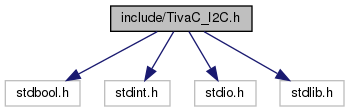
\includegraphics[width=334pt]{TivaC__I2C_8h__incl}
\end{center}
\end{figure}
This graph shows which files directly or indirectly include this file\+:\nopagebreak
\begin{figure}[H]
\begin{center}
\leavevmode
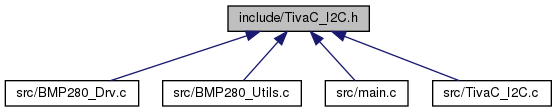
\includegraphics[width=350pt]{TivaC__I2C_8h__dep__incl}
\end{center}
\end{figure}
\subsection*{Macros}
\begin{DoxyCompactItemize}
\item 
\mbox{\Hypertarget{TivaC__I2C_8h_a7059148e07862aa60adee7cb5b86ae9d}\label{TivaC__I2C_8h_a7059148e07862aa60adee7cb5b86ae9d}} 
\#define {\bfseries R\+E\+M\+A\+I\+N\+\_\+\+T\+R\+A\+N\+S\+M\+IT}~2
\item 
\mbox{\Hypertarget{TivaC__I2C_8h_a8850ad3d7a751bc47f181a0bbcabf758}\label{TivaC__I2C_8h_a8850ad3d7a751bc47f181a0bbcabf758}} 
\#define {\bfseries N\+O\+\_\+\+R\+E\+M\+A\+I\+N\+\_\+\+T\+R\+A\+N\+S\+M\+IT}~0
\item 
\mbox{\Hypertarget{TivaC__I2C_8h_a6fd2714aedffacd7c401559c050a5012}\label{TivaC__I2C_8h_a6fd2714aedffacd7c401559c050a5012}} 
\#define {\bfseries R\+E\+M\+A\+I\+N\+\_\+\+R\+E\+C\+E\+I\+VE}~3
\item 
\mbox{\Hypertarget{TivaC__I2C_8h_a3c4f1937ce24883896a5861c7c959d9c}\label{TivaC__I2C_8h_a3c4f1937ce24883896a5861c7c959d9c}} 
\#define {\bfseries N\+O\+\_\+\+R\+E\+M\+A\+I\+N\+\_\+\+R\+E\+C\+E\+I\+VE}~0
\item 
\mbox{\Hypertarget{TivaC__I2C_8h_a14cf684224c0880a67ce1b260b787be3}\label{TivaC__I2C_8h_a14cf684224c0880a67ce1b260b787be3}} 
\#define {\bfseries N\+O\+\_\+\+R\+E\+P\+E\+A\+T\+\_\+\+S\+T\+A\+RT}~0
\item 
\mbox{\Hypertarget{TivaC__I2C_8h_a739044ea0313d14d019804ff5a41057d}\label{TivaC__I2C_8h_a739044ea0313d14d019804ff5a41057d}} 
\#define {\bfseries R\+E\+P\+E\+A\+T\+\_\+\+S\+T\+A\+RT}~1
\item 
\#define {\bfseries I2\+C0\+\_\+\+T\+R\+Y\+\_\+\+F\+U\+NC}(func\+To\+Execute)
\end{DoxyCompactItemize}
\subsection*{Enumerations}
\begin{DoxyCompactItemize}
\item 
\mbox{\Hypertarget{TivaC__I2C_8h_aa6338005075a5c377455028be821f224}\label{TivaC__I2C_8h_aa6338005075a5c377455028be821f224}} 
enum {\bfseries I2c0\+Err\+Code} \{ {\bfseries I2\+C0\+\_\+\+N\+O\+\_\+\+E\+RR} = 0, 
{\bfseries I2\+C0\+\_\+\+T\+I\+M\+E\+O\+UT}, 
{\bfseries I2\+C0\+\_\+\+B\+U\+S\+\_\+\+E\+R\+R\+OR}, 
{\bfseries I2\+C0\+\_\+\+M\+A\+S\+T\+E\+R\+\_\+\+D\+I\+S\+A\+B\+L\+ED}
 \}
\end{DoxyCompactItemize}
\subsection*{Functions}
\begin{DoxyCompactItemize}
\item 
\mbox{\Hypertarget{TivaC__I2C_8h_ab67308783773adc604bd5a0d87a511af}\label{TivaC__I2C_8h_ab67308783773adc604bd5a0d87a511af}} 
I2c0\+Err\+Code \hyperlink{TivaC__I2C_8h_ab67308783773adc604bd5a0d87a511af}{i2c0\+\_\+open} (void)
\begin{DoxyCompactList}\small\item\em enable clocks, I2C pins and calculate the appropriate clock period This function should be called first b4 any I2C operations \end{DoxyCompactList}\item 
\mbox{\Hypertarget{TivaC__I2C_8h_ad78ce9ab48b822965a2e58c0389edbd1}\label{TivaC__I2C_8h_ad78ce9ab48b822965a2e58c0389edbd1}} 
I2c0\+Err\+Code \hyperlink{TivaC__I2C_8h_ad78ce9ab48b822965a2e58c0389edbd1}{i2c0\+\_\+close} (void)
\begin{DoxyCompactList}\small\item\em Disable clock as well as the I2C pins. \end{DoxyCompactList}\item 
\mbox{\Hypertarget{TivaC__I2C_8h_ab9a581a005285f7e94a5c79d956f207b}\label{TivaC__I2C_8h_ab9a581a005285f7e94a5c79d956f207b}} 
I2c0\+Err\+Code \hyperlink{TivaC__I2C_8h_ab9a581a005285f7e94a5c79d956f207b}{i2c0\+\_\+stop} (void)
\begin{DoxyCompactList}\small\item\em used to generate I2C stop signal \end{DoxyCompactList}\item 
\mbox{\Hypertarget{TivaC__I2C_8h_ad6ba2e0d794a585e8f69ea37033971fa}\label{TivaC__I2C_8h_ad6ba2e0d794a585e8f69ea37033971fa}} 
I2c0\+Err\+Code \hyperlink{TivaC__I2C_8h_ad6ba2e0d794a585e8f69ea37033971fa}{i2c0\+\_\+keep\+\_\+state} (void)
\begin{DoxyCompactList}\small\item\em used to maintain current I2C state \end{DoxyCompactList}\item 
\mbox{\Hypertarget{TivaC__I2C_8h_af0bd7f3c3b91870a3b7616dd5d848365}\label{TivaC__I2C_8h_af0bd7f3c3b91870a3b7616dd5d848365}} 
I2c0\+Err\+Code \hyperlink{TivaC__I2C_8h_af0bd7f3c3b91870a3b7616dd5d848365}{i2c0\+\_\+multiple\+\_\+data\+\_\+byte\+\_\+write} (const uint8\+\_\+t slave\+\_\+address, const uint8\+\_\+t $\ast$output\+\_\+buffer, const uint8\+\_\+t output\+\_\+buffer\+\_\+length)
\begin{DoxyCompactList}\small\item\em write byte one by one until done \end{DoxyCompactList}\item 
\mbox{\Hypertarget{TivaC__I2C_8h_a8e258129956544f01ec903e3dd153454}\label{TivaC__I2C_8h_a8e258129956544f01ec903e3dd153454}} 
I2c0\+Err\+Code {\bfseries i2c0\+\_\+multiple\+\_\+data\+\_\+byte\+\_\+read} (const uint8\+\_\+t slave\+\_\+address, uint8\+\_\+t $\ast$input\+\_\+buffer, const uint8\+\_\+t input\+\_\+buffer\+\_\+length)
\item 
I2c0\+Err\+Code \hyperlink{TivaC__I2C_8h_ae51adb7272b1571ff425a124f0f5a7a5}{i2c0\+\_\+single\+\_\+data\+\_\+read} (const uint8\+\_\+t slave\+\_\+address, uint8\+\_\+t $\ast$return\+Data, const bool no\+\_\+ack, const bool no\+\_\+stop, const bool no\+\_\+start)
\begin{DoxyCompactList}\small\item\em read one byte of data \end{DoxyCompactList}\item 
I2c0\+Err\+Code \hyperlink{TivaC__I2C_8h_ab8c85ee87b4d758a3ff1bfbdbec6bf26}{i2c0\+\_\+single\+\_\+data\+\_\+write} (const uint8\+\_\+t slave\+\_\+address, const uint8\+\_\+t data\+\_\+byte, const bool no\+\_\+end\+\_\+stop)
\begin{DoxyCompactList}\small\item\em write a single byte using I2C \end{DoxyCompactList}\item 
\mbox{\Hypertarget{TivaC__I2C_8h_ab0f051ca77472369ee6bbb68b020f657}\label{TivaC__I2C_8h_ab0f051ca77472369ee6bbb68b020f657}} 
I2c0\+Err\+Code \hyperlink{TivaC__I2C_8h_ab0f051ca77472369ee6bbb68b020f657}{i2c0\+\_\+error\+\_\+check} (void)
\begin{DoxyCompactList}\small\item\em check i2c error register for any problems \end{DoxyCompactList}\item 
\mbox{\Hypertarget{TivaC__I2C_8h_a8cb69d8095fdbe6d8447f3413c280e03}\label{TivaC__I2C_8h_a8cb69d8095fdbe6d8447f3413c280e03}} 
I2c0\+Err\+Code \hyperlink{TivaC__I2C_8h_a8cb69d8095fdbe6d8447f3413c280e03}{i2c0\+\_\+check\+\_\+master\+\_\+enabled} (void)
\begin{DoxyCompactList}\small\item\em check i2c config register to see if the master functionality is enabled \end{DoxyCompactList}\item 
I2c0\+Err\+Code \hyperlink{TivaC__I2C_8h_ade2063cad2d3a4744d325dbbb3eda2c4}{i2c0\+\_\+wait\+\_\+bus} (void)
\begin{DoxyCompactList}\small\item\em used for waiting till the bus stops being busy \end{DoxyCompactList}\end{DoxyCompactItemize}


\subsection{Detailed Description}
contain i2c error enum and function prototypes 

\begin{DoxyAuthor}{Author}
Khoi Trinh 
\end{DoxyAuthor}
\begin{DoxyDate}{Date}
2018-\/08-\/25 
\end{DoxyDate}


\subsection{Macro Definition Documentation}
\mbox{\Hypertarget{TivaC__I2C_8h_a8297c9d9106a399efe4516ce9b323ddc}\label{TivaC__I2C_8h_a8297c9d9106a399efe4516ce9b323ddc}} 
\index{Tiva\+C\+\_\+\+I2\+C.\+h@{Tiva\+C\+\_\+\+I2\+C.\+h}!I2\+C0\+\_\+\+T\+R\+Y\+\_\+\+F\+U\+NC@{I2\+C0\+\_\+\+T\+R\+Y\+\_\+\+F\+U\+NC}}
\index{I2\+C0\+\_\+\+T\+R\+Y\+\_\+\+F\+U\+NC@{I2\+C0\+\_\+\+T\+R\+Y\+\_\+\+F\+U\+NC}!Tiva\+C\+\_\+\+I2\+C.\+h@{Tiva\+C\+\_\+\+I2\+C.\+h}}
\subsubsection{\texorpdfstring{I2\+C0\+\_\+\+T\+R\+Y\+\_\+\+F\+U\+NC}{I2C0\_TRY\_FUNC}}
{\footnotesize\ttfamily \#define I2\+C0\+\_\+\+T\+R\+Y\+\_\+\+F\+U\+NC(\begin{DoxyParamCaption}\item[{}]{func\+To\+Execute }\end{DoxyParamCaption})}

{\bfseries Value\+:}
\begin{DoxyCode}
\textcolor{keywordflow}{do} \{                                              \(\backslash\)
    I2c0ErrCode errCode = funcToExecute;            \(\backslash\)
    if (errCode != I2C0\_NO\_ERR) \{ \textcolor{keywordflow}{return} errCode; \} \(\backslash\)
  \} \textcolor{keywordflow}{while} (0)
\end{DoxyCode}


\subsection{Function Documentation}
\mbox{\Hypertarget{TivaC__I2C_8h_ae51adb7272b1571ff425a124f0f5a7a5}\label{TivaC__I2C_8h_ae51adb7272b1571ff425a124f0f5a7a5}} 
\index{Tiva\+C\+\_\+\+I2\+C.\+h@{Tiva\+C\+\_\+\+I2\+C.\+h}!i2c0\+\_\+single\+\_\+data\+\_\+read@{i2c0\+\_\+single\+\_\+data\+\_\+read}}
\index{i2c0\+\_\+single\+\_\+data\+\_\+read@{i2c0\+\_\+single\+\_\+data\+\_\+read}!Tiva\+C\+\_\+\+I2\+C.\+h@{Tiva\+C\+\_\+\+I2\+C.\+h}}
\subsubsection{\texorpdfstring{i2c0\+\_\+single\+\_\+data\+\_\+read()}{i2c0\_single\_data\_read()}}
{\footnotesize\ttfamily I2c0\+Err\+Code i2c0\+\_\+single\+\_\+data\+\_\+read (\begin{DoxyParamCaption}\item[{const uint8\+\_\+t}]{slave\+\_\+address,  }\item[{uint8\+\_\+t $\ast$}]{return\+Data,  }\item[{const bool}]{no\+\_\+ack,  }\item[{const bool}]{no\+\_\+stop,  }\item[{const bool}]{no\+\_\+start }\end{DoxyParamCaption})}



read one byte of data 


\begin{DoxyParams}{Parameters}
{\em no\+\_\+ack} & whether to generate ack signal \\
\hline
{\em no\+\_\+stop} & whether to generate stop signal \\
\hline
{\em no\+\_\+start} & whether to generate start(or repeated start) signal \\
\hline
\end{DoxyParams}
\mbox{\Hypertarget{TivaC__I2C_8h_ab8c85ee87b4d758a3ff1bfbdbec6bf26}\label{TivaC__I2C_8h_ab8c85ee87b4d758a3ff1bfbdbec6bf26}} 
\index{Tiva\+C\+\_\+\+I2\+C.\+h@{Tiva\+C\+\_\+\+I2\+C.\+h}!i2c0\+\_\+single\+\_\+data\+\_\+write@{i2c0\+\_\+single\+\_\+data\+\_\+write}}
\index{i2c0\+\_\+single\+\_\+data\+\_\+write@{i2c0\+\_\+single\+\_\+data\+\_\+write}!Tiva\+C\+\_\+\+I2\+C.\+h@{Tiva\+C\+\_\+\+I2\+C.\+h}}
\subsubsection{\texorpdfstring{i2c0\+\_\+single\+\_\+data\+\_\+write()}{i2c0\_single\_data\_write()}}
{\footnotesize\ttfamily I2c0\+Err\+Code i2c0\+\_\+single\+\_\+data\+\_\+write (\begin{DoxyParamCaption}\item[{const uint8\+\_\+t}]{slave\+\_\+address,  }\item[{const uint8\+\_\+t}]{data\+\_\+byte,  }\item[{const bool}]{no\+\_\+end\+\_\+stop }\end{DoxyParamCaption})}



write a single byte using I2C 


\begin{DoxyParams}{Parameters}
{\em no\+\_\+end\+\_\+stop} & whether to generate stop at the end of the write \\
\hline
\end{DoxyParams}
\mbox{\Hypertarget{TivaC__I2C_8h_ade2063cad2d3a4744d325dbbb3eda2c4}\label{TivaC__I2C_8h_ade2063cad2d3a4744d325dbbb3eda2c4}} 
\index{Tiva\+C\+\_\+\+I2\+C.\+h@{Tiva\+C\+\_\+\+I2\+C.\+h}!i2c0\+\_\+wait\+\_\+bus@{i2c0\+\_\+wait\+\_\+bus}}
\index{i2c0\+\_\+wait\+\_\+bus@{i2c0\+\_\+wait\+\_\+bus}!Tiva\+C\+\_\+\+I2\+C.\+h@{Tiva\+C\+\_\+\+I2\+C.\+h}}
\subsubsection{\texorpdfstring{i2c0\+\_\+wait\+\_\+bus()}{i2c0\_wait\_bus()}}
{\footnotesize\ttfamily I2c0\+Err\+Code i2c0\+\_\+wait\+\_\+bus (\begin{DoxyParamCaption}\item[{void}]{ }\end{DoxyParamCaption})}



used for waiting till the bus stops being busy 

\begin{DoxyReturn}{Returns}
whether the bus is idle now or timeout happened 
\end{DoxyReturn}

\hypertarget{TivaC__SPI_8h}{}\section{include/\+Tiva\+C\+\_\+\+S\+PI.h File Reference}
\label{TivaC__SPI_8h}\index{include/\+Tiva\+C\+\_\+\+S\+P\+I.\+h@{include/\+Tiva\+C\+\_\+\+S\+P\+I.\+h}}


contain data structure for S\+PI settings, errors as well as enum for various settings  


{\ttfamily \#include $<$stdbool.\+h$>$}\newline
{\ttfamily \#include $<$stdint.\+h$>$}\newline
Include dependency graph for Tiva\+C\+\_\+\+S\+P\+I.\+h\+:\nopagebreak
\begin{figure}[H]
\begin{center}
\leavevmode
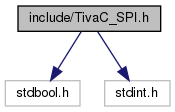
\includegraphics[width=204pt]{TivaC__SPI_8h__incl}
\end{center}
\end{figure}
This graph shows which files directly or indirectly include this file\+:\nopagebreak
\begin{figure}[H]
\begin{center}
\leavevmode
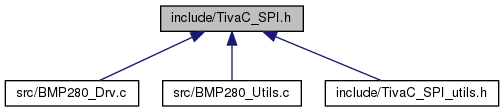
\includegraphics[width=350pt]{TivaC__SPI_8h__dep__incl}
\end{center}
\end{figure}
\subsection*{Data Structures}
\begin{DoxyCompactItemize}
\item 
struct \hyperlink{structSpiSettings}{Spi\+Settings}
\begin{DoxyCompactList}\small\item\em represent a spi module \end{DoxyCompactList}\end{DoxyCompactItemize}
\subsection*{Macros}
\begin{DoxyCompactItemize}
\item 
\mbox{\Hypertarget{TivaC__SPI_8h_ac4a8cec2cfd0d3fd322fb27149af0fd5}\label{TivaC__SPI_8h_ac4a8cec2cfd0d3fd322fb27149af0fd5}} 
\#define \hyperlink{TivaC__SPI_8h_ac4a8cec2cfd0d3fd322fb27149af0fd5}{S\+P\+I\+\_\+\+T\+R\+F\+\_\+\+S\+I\+ZE}~8
\begin{DoxyCompactList}\small\item\em the smallest transfer size of the spi, note that this is different from the transfer size in the spi structure, a complete transfer is made up of small 8 bit transfers \end{DoxyCompactList}\item 
\#define {\bfseries S\+P\+I\+\_\+\+T\+R\+Y\+\_\+\+F\+U\+NC}(func\+To\+Execute)
\end{DoxyCompactItemize}
\subsection*{Enumerations}
\begin{DoxyCompactItemize}
\item 
\mbox{\Hypertarget{TivaC__SPI_8h_a3a4379fe5892fb16c076de874ac889db}\label{TivaC__SPI_8h_a3a4379fe5892fb16c076de874ac889db}} 
enum \hyperlink{TivaC__SPI_8h_a3a4379fe5892fb16c076de874ac889db}{Spi\+Err\+Code} \{ \newline
{\bfseries S\+P\+I\+\_\+\+E\+R\+R\+\_\+\+N\+O\+\_\+\+E\+RR}, 
{\bfseries S\+P\+I\+\_\+\+E\+R\+R\+\_\+\+D\+I\+S\+A\+B\+L\+ED}, 
{\bfseries S\+P\+I\+\_\+\+E\+R\+R\+\_\+\+T\+I\+M\+E\+O\+UT}, 
{\bfseries S\+P\+I\+\_\+\+E\+R\+R\+\_\+\+S\+P\+I\+\_\+\+C\+P\+A\+\_\+\+U\+N\+D\+E\+F\+I\+N\+ED}, 
\newline
{\bfseries S\+P\+I\+\_\+\+E\+R\+R\+\_\+\+R\+X\+\_\+\+F\+U\+LL}, 
{\bfseries S\+P\+I\+\_\+\+E\+R\+R\+\_\+\+T\+X\+\_\+\+F\+U\+LL}, 
{\bfseries S\+P\+I\+\_\+\+E\+R\+R\+\_\+\+R\+X\+\_\+\+E\+M\+P\+TY}, 
{\bfseries S\+P\+I\+\_\+\+E\+R\+R\+\_\+\+I\+N\+V\+A\+L\+\_\+\+S\+Y\+S\+\_\+\+C\+L\+K\+\_\+\+R\+A\+TE}, 
\newline
{\bfseries S\+P\+I\+\_\+\+E\+R\+R\+\_\+\+N\+O\+\_\+\+V\+A\+L\+\_\+\+P\+R\+E\+S\+C\+A\+LC}, 
{\bfseries S\+P\+I\+\_\+\+E\+R\+R\+\_\+\+I\+N\+V\+A\+L\+\_\+\+B\+I\+T\+\_\+\+R\+A\+TE}, 
{\bfseries S\+P\+I\+\_\+\+E\+R\+R\+\_\+\+I\+N\+V\+A\+L\+\_\+\+D\+A\+T\+A\+\_\+\+S\+I\+ZE}, 
{\bfseries S\+P\+I\+\_\+\+E\+R\+R\+\_\+\+I\+N\+V\+A\+L\+\_\+\+C\+P\+OL}, 
\newline
{\bfseries S\+P\+I\+\_\+\+E\+R\+R\+\_\+\+I\+N\+V\+A\+L\+\_\+\+C\+P\+HA}, 
{\bfseries S\+P\+I\+\_\+\+E\+R\+R\+\_\+\+I\+N\+V\+A\+L\+\_\+\+P\+R\+O\+T\+O\+C\+OL}, 
{\bfseries S\+P\+I\+\_\+\+E\+R\+R\+\_\+\+I\+N\+V\+A\+L\+\_\+\+R\+O\+LE}, 
{\bfseries S\+P\+I\+\_\+\+E\+R\+R\+\_\+\+I\+N\+V\+A\+L\+\_\+\+O\+P\+E\+R\+M\+O\+DE}, 
\newline
{\bfseries S\+P\+I\+\_\+\+E\+R\+R\+\_\+\+I\+N\+V\+A\+L\+\_\+\+C\+L\+O\+C\+K\+S\+O\+U\+R\+CE}
 \}\begin{DoxyCompactList}\small\item\em S\+PI error code. \end{DoxyCompactList}
\item 
\mbox{\Hypertarget{TivaC__SPI_8h_aa453f368264f8e25288c765016fe682e}\label{TivaC__SPI_8h_aa453f368264f8e25288c765016fe682e}} 
enum {\bfseries Spi\+Protocol\+Mode} \{ {\bfseries Freescale}, 
{\bfseries Tissf}, 
{\bfseries Microwire}
 \}
\item 
\mbox{\Hypertarget{TivaC__SPI_8h_a7fa0276fb58c61168e098931d9471bb7}\label{TivaC__SPI_8h_a7fa0276fb58c61168e098931d9471bb7}} 
enum {\bfseries Spi\+Role} \{ {\bfseries Slave}, 
{\bfseries Master}
 \}
\item 
\mbox{\Hypertarget{TivaC__SPI_8h_acf1a803586170334621a9a55e90a2ffb}\label{TivaC__SPI_8h_acf1a803586170334621a9a55e90a2ffb}} 
enum {\bfseries Clock\+Source} \{ {\bfseries Systemclock}, 
{\bfseries Piosc}
 \}
\end{DoxyCompactItemize}
\subsection*{Functions}
\begin{DoxyCompactItemize}
\item 
\hyperlink{TivaC__SPI_8h_a3a4379fe5892fb16c076de874ac889db}{Spi\+Err\+Code} \hyperlink{TivaC__SPI_8h_a12b73afd32ec56549a49243d61154740}{spi\+\_\+open} (const \hyperlink{structSpiSettings}{Spi\+Settings} setting)
\begin{DoxyCompactList}\small\item\em set up spi bus, should be called first \end{DoxyCompactList}\item 
\hyperlink{TivaC__SPI_8h_a3a4379fe5892fb16c076de874ac889db}{Spi\+Err\+Code} \hyperlink{TivaC__SPI_8h_a8203f5d7ead72b1a5f4f6336a7e67bcc}{spi\+\_\+close} (void)
\begin{DoxyCompactList}\small\item\em turn off clock for the S\+PI module \end{DoxyCompactList}\item 
\mbox{\Hypertarget{TivaC__SPI_8h_a782c68fc08576e31fa6a03218bed8396}\label{TivaC__SPI_8h_a782c68fc08576e31fa6a03218bed8396}} 
\hyperlink{TivaC__SPI_8h_a3a4379fe5892fb16c076de874ac889db}{Spi\+Err\+Code} \hyperlink{TivaC__SPI_8h_a782c68fc08576e31fa6a03218bed8396}{spi\+\_\+check\+\_\+spi\+\_\+enabled} (void)
\begin{DoxyCompactList}\small\item\em check if the clock for S\+PI is turned on \end{DoxyCompactList}\item 
\hyperlink{TivaC__SPI_8h_a3a4379fe5892fb16c076de874ac889db}{Spi\+Err\+Code} \hyperlink{TivaC__SPI_8h_a11a9f3594b3e76f05cdcdb2146d1f99c}{spi\+\_\+transfer} (const \hyperlink{structSpiSettings}{Spi\+Settings} setting, uint8\+\_\+t $\ast$data\+Tx, const uint8\+\_\+t data\+Tx\+Len\+Byte, uint8\+\_\+t $\ast$data\+Rx, const uint8\+\_\+t data\+Rx\+Len\+Byte)
\begin{DoxyCompactList}\small\item\em used for both rx and tx \end{DoxyCompactList}\end{DoxyCompactItemize}


\subsection{Detailed Description}
contain data structure for S\+PI settings, errors as well as enum for various settings 

\begin{DoxyAuthor}{Author}
Khoi Trinh 
\end{DoxyAuthor}
\begin{DoxyDate}{Date}
2018-\/08-\/25 
\end{DoxyDate}


\subsection{Macro Definition Documentation}
\mbox{\Hypertarget{TivaC__SPI_8h_afc7a246bd787cd6acfd93b7649137c34}\label{TivaC__SPI_8h_afc7a246bd787cd6acfd93b7649137c34}} 
\index{Tiva\+C\+\_\+\+S\+P\+I.\+h@{Tiva\+C\+\_\+\+S\+P\+I.\+h}!S\+P\+I\+\_\+\+T\+R\+Y\+\_\+\+F\+U\+NC@{S\+P\+I\+\_\+\+T\+R\+Y\+\_\+\+F\+U\+NC}}
\index{S\+P\+I\+\_\+\+T\+R\+Y\+\_\+\+F\+U\+NC@{S\+P\+I\+\_\+\+T\+R\+Y\+\_\+\+F\+U\+NC}!Tiva\+C\+\_\+\+S\+P\+I.\+h@{Tiva\+C\+\_\+\+S\+P\+I.\+h}}
\subsubsection{\texorpdfstring{S\+P\+I\+\_\+\+T\+R\+Y\+\_\+\+F\+U\+NC}{SPI\_TRY\_FUNC}}
{\footnotesize\ttfamily \#define S\+P\+I\+\_\+\+T\+R\+Y\+\_\+\+F\+U\+NC(\begin{DoxyParamCaption}\item[{}]{func\+To\+Execute }\end{DoxyParamCaption})}

{\bfseries Value\+:}
\begin{DoxyCode}
\textcolor{keywordflow}{do} \{                                                 \(\backslash\)
    SpiErrCode errCode = funcToExecute;                \(\backslash\)
    if (errCode != SPI\_ERR\_NO\_ERR) \{ \textcolor{keywordflow}{return} errCode; \} \(\backslash\)
  \} \textcolor{keywordflow}{while} (0)
\end{DoxyCode}


\subsection{Function Documentation}
\mbox{\Hypertarget{TivaC__SPI_8h_a8203f5d7ead72b1a5f4f6336a7e67bcc}\label{TivaC__SPI_8h_a8203f5d7ead72b1a5f4f6336a7e67bcc}} 
\index{Tiva\+C\+\_\+\+S\+P\+I.\+h@{Tiva\+C\+\_\+\+S\+P\+I.\+h}!spi\+\_\+close@{spi\+\_\+close}}
\index{spi\+\_\+close@{spi\+\_\+close}!Tiva\+C\+\_\+\+S\+P\+I.\+h@{Tiva\+C\+\_\+\+S\+P\+I.\+h}}
\subsubsection{\texorpdfstring{spi\+\_\+close()}{spi\_close()}}
{\footnotesize\ttfamily \hyperlink{TivaC__SPI_8h_a3a4379fe5892fb16c076de874ac889db}{Spi\+Err\+Code} spi\+\_\+close (\begin{DoxyParamCaption}\item[{void}]{ }\end{DoxyParamCaption})}



turn off clock for the S\+PI module 

Will wait to make sure that all S\+PI traffic is done before turning off the clock \mbox{\Hypertarget{TivaC__SPI_8h_a12b73afd32ec56549a49243d61154740}\label{TivaC__SPI_8h_a12b73afd32ec56549a49243d61154740}} 
\index{Tiva\+C\+\_\+\+S\+P\+I.\+h@{Tiva\+C\+\_\+\+S\+P\+I.\+h}!spi\+\_\+open@{spi\+\_\+open}}
\index{spi\+\_\+open@{spi\+\_\+open}!Tiva\+C\+\_\+\+S\+P\+I.\+h@{Tiva\+C\+\_\+\+S\+P\+I.\+h}}
\subsubsection{\texorpdfstring{spi\+\_\+open()}{spi\_open()}}
{\footnotesize\ttfamily \hyperlink{TivaC__SPI_8h_a3a4379fe5892fb16c076de874ac889db}{Spi\+Err\+Code} spi\+\_\+open (\begin{DoxyParamCaption}\item[{const \hyperlink{structSpiSettings}{Spi\+Settings}}]{setting }\end{DoxyParamCaption})}



set up spi bus, should be called first 

used to turn on the clock, adjust the S\+PI pins and apply all the users settings to the S\+PI modules, note that the S\+PI module would still be off after this function but it only needs to be enabled to function \mbox{\Hypertarget{TivaC__SPI_8h_a11a9f3594b3e76f05cdcdb2146d1f99c}\label{TivaC__SPI_8h_a11a9f3594b3e76f05cdcdb2146d1f99c}} 
\index{Tiva\+C\+\_\+\+S\+P\+I.\+h@{Tiva\+C\+\_\+\+S\+P\+I.\+h}!spi\+\_\+transfer@{spi\+\_\+transfer}}
\index{spi\+\_\+transfer@{spi\+\_\+transfer}!Tiva\+C\+\_\+\+S\+P\+I.\+h@{Tiva\+C\+\_\+\+S\+P\+I.\+h}}
\subsubsection{\texorpdfstring{spi\+\_\+transfer()}{spi\_transfer()}}
{\footnotesize\ttfamily \hyperlink{TivaC__SPI_8h_a3a4379fe5892fb16c076de874ac889db}{Spi\+Err\+Code} spi\+\_\+transfer (\begin{DoxyParamCaption}\item[{const \hyperlink{structSpiSettings}{Spi\+Settings}}]{setting,  }\item[{uint8\+\_\+t $\ast$}]{data\+Tx,  }\item[{const uint8\+\_\+t}]{data\+Tx\+Len\+Byte,  }\item[{uint8\+\_\+t $\ast$}]{data\+Rx,  }\item[{const uint8\+\_\+t}]{data\+Rx\+Len\+Byte }\end{DoxyParamCaption})}



used for both rx and tx 

enable S\+PI, and then send/receive based on the user inputs, after a transfer the S\+PI module would be disabled to make sure no transfer erroneously happens, this is a soft disable with all the clocks and pins still S\+P\+I-\/ready 
\hypertarget{TivaC__SPI__utils_8h}{}\section{include/\+Tiva\+C\+\_\+\+S\+P\+I\+\_\+utils.h File Reference}
\label{TivaC__SPI__utils_8h}\index{include/\+Tiva\+C\+\_\+\+S\+P\+I\+\_\+utils.\+h@{include/\+Tiva\+C\+\_\+\+S\+P\+I\+\_\+utils.\+h}}


header file for S\+PI utilities functions  


{\ttfamily \#include $<$stdint.\+h$>$}\newline
{\ttfamily \#include \char`\"{}include/\+Tiva\+C\+\_\+\+S\+P\+I.\+h\char`\"{}}\newline
{\ttfamily \#include \char`\"{}include/tm4c123gh6pm.\+h\char`\"{}}\newline
Include dependency graph for Tiva\+C\+\_\+\+S\+P\+I\+\_\+utils.\+h\+:\nopagebreak
\begin{figure}[H]
\begin{center}
\leavevmode
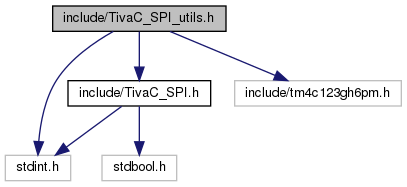
\includegraphics[width=350pt]{TivaC__SPI__utils_8h__incl}
\end{center}
\end{figure}
\subsection*{Functions}
\begin{DoxyCompactItemize}
\item 
\mbox{\Hypertarget{TivaC__SPI__utils_8h_a75e2e39f095c5aed9f1404209f41ea2f}\label{TivaC__SPI__utils_8h_a75e2e39f095c5aed9f1404209f41ea2f}} 
\hyperlink{TivaC__SPI_8h_a3a4379fe5892fb16c076de874ac889db}{Spi\+Err\+Code} \hyperlink{TivaC__SPI__utils_8h_a75e2e39f095c5aed9f1404209f41ea2f}{spi\+\_\+check\+\_\+setting} (const \hyperlink{structSpiSettings}{Spi\+Settings} setting)
\begin{DoxyCompactList}\small\item\em check user settings to see if they are logical \end{DoxyCompactList}\item 
\mbox{\Hypertarget{TivaC__SPI__utils_8h_ad13f4a862a1214c17eba3e1a30e606b8}\label{TivaC__SPI__utils_8h_ad13f4a862a1214c17eba3e1a30e606b8}} 
\hyperlink{TivaC__SPI_8h_a3a4379fe5892fb16c076de874ac889db}{Spi\+Err\+Code} {\bfseries spi\+\_\+check\+\_\+rx\+\_\+full} (void)
\item 
\mbox{\Hypertarget{TivaC__SPI__utils_8h_a4dd6f46726dae4cd86785f36bc28a064}\label{TivaC__SPI__utils_8h_a4dd6f46726dae4cd86785f36bc28a064}} 
\hyperlink{TivaC__SPI_8h_a3a4379fe5892fb16c076de874ac889db}{Spi\+Err\+Code} {\bfseries spi\+\_\+check\+\_\+tx\+\_\+full} (void)
\item 
\mbox{\Hypertarget{TivaC__SPI__utils_8h_ac33fc00ccd26b1cb75a6fabc7efc4839}\label{TivaC__SPI__utils_8h_ac33fc00ccd26b1cb75a6fabc7efc4839}} 
\hyperlink{TivaC__SPI_8h_a3a4379fe5892fb16c076de874ac889db}{Spi\+Err\+Code} {\bfseries spi\+\_\+check\+\_\+rx\+\_\+not\+\_\+empty} (void)
\item 
\hyperlink{TivaC__SPI_8h_a3a4379fe5892fb16c076de874ac889db}{Spi\+Err\+Code} \hyperlink{TivaC__SPI__utils_8h_a1aa8e59f77487dd762878eeeb136bea3}{spi\+\_\+calc\+\_\+clock\+\_\+prescalc} (const \hyperlink{structSpiSettings}{Spi\+Settings} setting, uint8\+\_\+t $\ast$pre\+Scalc, uint8\+\_\+t $\ast$scr)
\begin{DoxyCompactList}\small\item\em calculate spi clock prescaler number \end{DoxyCompactList}\item 
\mbox{\Hypertarget{TivaC__SPI__utils_8h_a5b03049a2c7efe2fec01007cef275e40}\label{TivaC__SPI__utils_8h_a5b03049a2c7efe2fec01007cef275e40}} 
\hyperlink{TivaC__SPI_8h_a3a4379fe5892fb16c076de874ac889db}{Spi\+Err\+Code} \hyperlink{TivaC__SPI__utils_8h_a5b03049a2c7efe2fec01007cef275e40}{spi\+\_\+bus\+\_\+wait} (void)
\begin{DoxyCompactList}\small\item\em wait until the spi bus is not busy anymore \end{DoxyCompactList}\item 
\mbox{\Hypertarget{TivaC__SPI__utils_8h_a917d6dec06c1a5f4204a94121f1566d3}\label{TivaC__SPI__utils_8h_a917d6dec06c1a5f4204a94121f1566d3}} 
void \hyperlink{TivaC__SPI__utils_8h_a917d6dec06c1a5f4204a94121f1566d3}{spi\+\_\+enable\+\_\+spi} (void)
\begin{DoxyCompactList}\small\item\em enable spi modules, note that this is different from turning on the clock, this assumes that the clock is turn on and all pins are S\+P\+I-\/ready \end{DoxyCompactList}\item 
\mbox{\Hypertarget{TivaC__SPI__utils_8h_a126ecd9fffb497ae45b83ef92b925075}\label{TivaC__SPI__utils_8h_a126ecd9fffb497ae45b83ef92b925075}} 
void \hyperlink{TivaC__SPI__utils_8h_a126ecd9fffb497ae45b83ef92b925075}{spi\+\_\+disable\+\_\+spi} (void)
\begin{DoxyCompactList}\small\item\em disable spi modules, but leave the S\+PI clocks and pins still S\+P\+I-\/ready \end{DoxyCompactList}\item 
\mbox{\Hypertarget{TivaC__SPI__utils_8h_ad2e3a01d42741e9a944843dfd2403777}\label{TivaC__SPI__utils_8h_ad2e3a01d42741e9a944843dfd2403777}} 
void \hyperlink{TivaC__SPI__utils_8h_ad2e3a01d42741e9a944843dfd2403777}{spi\+\_\+pull\+\_\+cs\+\_\+low} (void)
\begin{DoxyCompactList}\small\item\em pull chip select pin low to activate S\+PI, hardcoded to be pin 3 of port A \end{DoxyCompactList}\item 
\mbox{\Hypertarget{TivaC__SPI__utils_8h_aebcad4e2f1d2721b28041e33984ca143}\label{TivaC__SPI__utils_8h_aebcad4e2f1d2721b28041e33984ca143}} 
void {\bfseries spi\+\_\+pull\+\_\+cs\+\_\+high} (void)
\item 
\mbox{\Hypertarget{TivaC__SPI__utils_8h_a25f68c7ccbe2aa563848fef9ae783997}\label{TivaC__SPI__utils_8h_a25f68c7ccbe2aa563848fef9ae783997}} 
\hyperlink{TivaC__SPI_8h_a3a4379fe5892fb16c076de874ac889db}{Spi\+Err\+Code} \hyperlink{TivaC__SPI__utils_8h_a25f68c7ccbe2aa563848fef9ae783997}{spi\+\_\+send\+\_\+dummy\+\_\+byte} (void)
\begin{DoxyCompactList}\small\item\em used for sending byte 0 to extend the S\+PI communication, usually to finish reading all the bytes that users want \end{DoxyCompactList}\item 
\mbox{\Hypertarget{TivaC__SPI__utils_8h_ab640efbed4dd7ffb7c30a3d883a4038e}\label{TivaC__SPI__utils_8h_ab640efbed4dd7ffb7c30a3d883a4038e}} 
void {\bfseries spi\+\_\+data\+\_\+delay} (void)
\item 
\mbox{\Hypertarget{TivaC__SPI__utils_8h_acd2cbe40a14e1694b6dc217fabf96d66}\label{TivaC__SPI__utils_8h_acd2cbe40a14e1694b6dc217fabf96d66}} 
\hyperlink{TivaC__SPI_8h_a3a4379fe5892fb16c076de874ac889db}{Spi\+Err\+Code} \hyperlink{TivaC__SPI__utils_8h_acd2cbe40a14e1694b6dc217fabf96d66}{spi\+\_\+rx\+\_\+one\+\_\+data\+\_\+unit} (const \hyperlink{structSpiSettings}{Spi\+Settings} setting, uint8\+\_\+t $\ast$total\+Byte\+Rxed, uint8\+\_\+t $\ast$data\+Rx)
\begin{DoxyCompactList}\small\item\em receive one data unit from the S\+PI buffer \end{DoxyCompactList}\item 
\mbox{\Hypertarget{TivaC__SPI__utils_8h_ac60b29ad366c6edd9a876ab6d801cf02}\label{TivaC__SPI__utils_8h_ac60b29ad366c6edd9a876ab6d801cf02}} 
\hyperlink{TivaC__SPI_8h_a3a4379fe5892fb16c076de874ac889db}{Spi\+Err\+Code} \hyperlink{TivaC__SPI__utils_8h_ac60b29ad366c6edd9a876ab6d801cf02}{spi\+\_\+tx\+\_\+one\+\_\+data\+\_\+unit} (const uint8\+\_\+t transfer\+Size, uint8\+\_\+t $\ast$total\+Byte\+Txed, const uint8\+\_\+t $\ast$data\+Tx)
\begin{DoxyCompactList}\small\item\em send 8 bits of data on the S\+PI interface \end{DoxyCompactList}\item 
\mbox{\Hypertarget{TivaC__SPI__utils_8h_a6745a65c6abffa7de06e25252dfa5689}\label{TivaC__SPI__utils_8h_a6745a65c6abffa7de06e25252dfa5689}} 
void {\bfseries spi\+\_\+clear\+\_\+rx\+\_\+buffer} (void)
\end{DoxyCompactItemize}


\subsection{Detailed Description}
header file for S\+PI utilities functions 

\begin{DoxyAuthor}{Author}
Khoi Trinh 
\end{DoxyAuthor}
\begin{DoxyDate}{Date}
2018-\/08-\/25 
\end{DoxyDate}


\subsection{Function Documentation}
\mbox{\Hypertarget{TivaC__SPI__utils_8h_a1aa8e59f77487dd762878eeeb136bea3}\label{TivaC__SPI__utils_8h_a1aa8e59f77487dd762878eeeb136bea3}} 
\index{Tiva\+C\+\_\+\+S\+P\+I\+\_\+utils.\+h@{Tiva\+C\+\_\+\+S\+P\+I\+\_\+utils.\+h}!spi\+\_\+calc\+\_\+clock\+\_\+prescalc@{spi\+\_\+calc\+\_\+clock\+\_\+prescalc}}
\index{spi\+\_\+calc\+\_\+clock\+\_\+prescalc@{spi\+\_\+calc\+\_\+clock\+\_\+prescalc}!Tiva\+C\+\_\+\+S\+P\+I\+\_\+utils.\+h@{Tiva\+C\+\_\+\+S\+P\+I\+\_\+utils.\+h}}
\subsubsection{\texorpdfstring{spi\+\_\+calc\+\_\+clock\+\_\+prescalc()}{spi\_calc\_clock\_prescalc()}}
{\footnotesize\ttfamily \hyperlink{TivaC__SPI_8h_a3a4379fe5892fb16c076de874ac889db}{Spi\+Err\+Code} spi\+\_\+calc\+\_\+clock\+\_\+prescalc (\begin{DoxyParamCaption}\item[{const \hyperlink{structSpiSettings}{Spi\+Settings}}]{setting,  }\item[{uint8\+\_\+t $\ast$}]{pre\+Scalc,  }\item[{uint8\+\_\+t $\ast$}]{scr }\end{DoxyParamCaption})}



calculate spi clock prescaler number 


\begin{DoxyParams}{Parameters}
{\em pre\+Scalc} & the calculated prescaler value \\
\hline
{\em scr} & the desired serial clock rate \\
\hline
\end{DoxyParams}
\begin{DoxyReturn}{Returns}
whether it\textquotesingle{}s possible to find a prescaler value for the specific scr 
\end{DoxyReturn}

\hypertarget{BMP280__Drv_8c}{}\section{src/\+B\+M\+P280\+\_\+\+Drv.c File Reference}
\label{BMP280__Drv_8c}\index{src/\+B\+M\+P280\+\_\+\+Drv.\+c@{src/\+B\+M\+P280\+\_\+\+Drv.\+c}}


Driver files, contain the top layer of the B\+M\+P280 A\+PI, contains ideally no I2C or S\+PI specific stuffs.  


{\ttfamily \#include \char`\"{}include/\+B\+M\+P280\+\_\+\+Drv.\+h\char`\"{}}\newline
{\ttfamily \#include $<$assert.\+h$>$}\newline
{\ttfamily \#include $<$stdbool.\+h$>$}\newline
{\ttfamily \#include \char`\"{}external/\+Tiva\+C\+\_\+\+Utils/include/\+Tiva\+C\+\_\+\+Other\+\_\+\+Utils.\+h\char`\"{}}\newline
{\ttfamily \#include \char`\"{}external/\+Tiva\+C\+\_\+\+Utils/include/bit\+\_\+manipulation.\+h\char`\"{}}\newline
{\ttfamily \#include \char`\"{}include/\+B\+M\+P280\+\_\+\+Utils.\+h\char`\"{}}\newline
{\ttfamily \#include \char`\"{}include/\+B\+M\+P280\+\_\+\+Ware.\+h\char`\"{}}\newline
{\ttfamily \#include \char`\"{}include/\+Tiva\+C\+\_\+\+I2\+C.\+h\char`\"{}}\newline
{\ttfamily \#include \char`\"{}include/\+Tiva\+C\+\_\+\+S\+P\+I.\+h\char`\"{}}\newline
Include dependency graph for B\+M\+P280\+\_\+\+Drv.\+c\+:\nopagebreak
\begin{figure}[H]
\begin{center}
\leavevmode
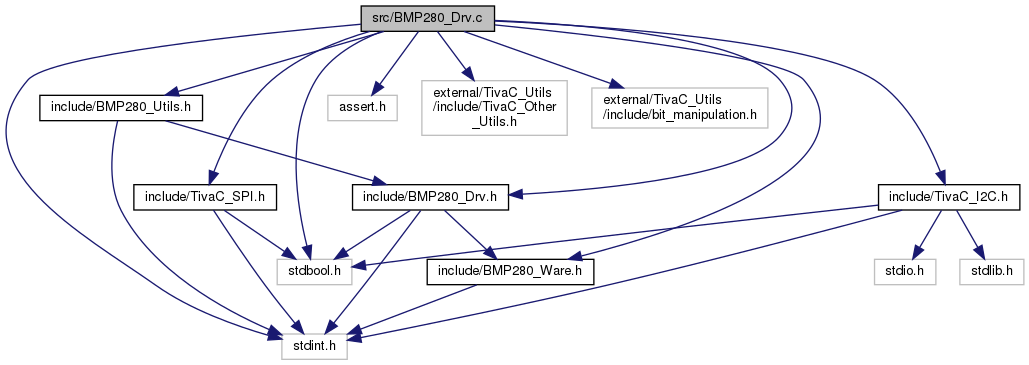
\includegraphics[width=350pt]{BMP280__Drv_8c__incl}
\end{center}
\end{figure}
\subsection*{Macros}
\begin{DoxyCompactItemize}
\item 
\mbox{\Hypertarget{BMP280__Drv_8c_a3323e52608dc9b1bd97b8e71e7c44f62}\label{BMP280__Drv_8c_a3323e52608dc9b1bd97b8e71e7c44f62}} 
\#define {\bfseries B\+M\+P280\+\_\+\+B\+A\+S\+E\+A\+D\+DR}~0x\+F3
\item 
\mbox{\Hypertarget{BMP280__Drv_8c_ac1d9dbd7e41f32c0cb0923c7d4fd8f97}\label{BMP280__Drv_8c_ac1d9dbd7e41f32c0cb0923c7d4fd8f97}} 
\#define {\bfseries R\+A\+W\+\_\+\+T\+E\+M\+\_\+\+T\+O\+T\+A\+L\+\_\+\+B\+Y\+TE}~3
\item 
\mbox{\Hypertarget{BMP280__Drv_8c_abd8baeeaa077ad9bffdd4cf9651be313}\label{BMP280__Drv_8c_abd8baeeaa077ad9bffdd4cf9651be313}} 
\#define {\bfseries R\+A\+W\+\_\+\+P\+R\+E\+S\+S\+\_\+\+T\+O\+T\+A\+L\+\_\+\+B\+Y\+TE}~3
\item 
\mbox{\Hypertarget{BMP280__Drv_8c_ad2356a4e2882a4c8c64cb635327ee892}\label{BMP280__Drv_8c_ad2356a4e2882a4c8c64cb635327ee892}} 
\#define {\bfseries B\+M\+P280\+\_\+\+C\+A\+L\+I\+B\+\_\+\+S\+T\+A\+R\+T\+\_\+\+A\+D\+DR}~0x88
\item 
\mbox{\Hypertarget{BMP280__Drv_8c_adc285c2e63f48773a076aada5b897e06}\label{BMP280__Drv_8c_adc285c2e63f48773a076aada5b897e06}} 
\#define {\bfseries B\+M\+P280\+\_\+\+R\+E\+S\+A\+D\+DR}~0x\+E0
\item 
\mbox{\Hypertarget{BMP280__Drv_8c_a7352d96b04a72365a99aa79ba14e7c49}\label{BMP280__Drv_8c_a7352d96b04a72365a99aa79ba14e7c49}} 
\#define {\bfseries B\+M\+P280\+\_\+\+I\+D\+A\+RR}~0x\+D0
\item 
\mbox{\Hypertarget{BMP280__Drv_8c_a5c988c599f3e498f853ef7f7e8e78ae4}\label{BMP280__Drv_8c_a5c988c599f3e498f853ef7f7e8e78ae4}} 
\#define {\bfseries B\+M\+P280\+\_\+\+M\+E\+A\+S\+U\+R\+I\+N\+G\+\_\+\+M\+A\+SK}~0x8
\item 
\mbox{\Hypertarget{BMP280__Drv_8c_a1f500317eb84c3e350021d319ab982f6}\label{BMP280__Drv_8c_a1f500317eb84c3e350021d319ab982f6}} 
\#define {\bfseries B\+M\+P280\+\_\+\+U\+P\+D\+A\+T\+I\+N\+G\+\_\+\+M\+A\+SK}~0x1
\end{DoxyCompactItemize}
\subsection*{Enumerations}
\begin{DoxyCompactItemize}
\item 
\mbox{\Hypertarget{BMP280__Drv_8c_acfc9e3a58bd723695e6ada7e5c8abd80}\label{BMP280__Drv_8c_acfc9e3a58bd723695e6ada7e5c8abd80}} 
enum {\bfseries bmp280\+\_\+reg\+Name} \{ \newline
{\bfseries Status} = 0, 
{\bfseries Ctrl\+\_\+meas}, 
{\bfseries Config}, 
{\bfseries Press\+\_\+msb} = 4, 
\newline
{\bfseries Press\+\_\+lsb}, 
{\bfseries Press\+\_\+xlsb}, 
{\bfseries Temp\+\_\+msb}, 
{\bfseries Temp\+\_\+lsb}, 
\newline
{\bfseries Temp\+\_\+xlsb}
 \}
\end{DoxyCompactItemize}
\subsection*{Functions}
\begin{DoxyCompactItemize}
\item 
\hyperlink{BMP280__Drv_8h_a726300a3932e443ece00fcc5c4f3ca7c}{Bmp280\+Err\+Code} \hyperlink{BMP280__Drv_8c_a688a1cfffa854195e06f133867897012}{bmp280\+\_\+create\+\_\+predefined\+\_\+settings} (\hyperlink{BMP280__Drv_8h_ab9e22f3267ce8af4053eb1189db84627}{bmp280} $\ast$sensor, const \hyperlink{BMP280__Drv_8h_a4a0fcacff61a12b6888fc060fc2baddb}{Bmp280\+Measure\+Settings} settings)
\begin{DoxyCompactList}\small\item\em initialize the bmp280 with predefined value in the datasheet \end{DoxyCompactList}\item 
\hyperlink{BMP280__Drv_8h_a726300a3932e443ece00fcc5c4f3ca7c}{Bmp280\+Err\+Code} \hyperlink{BMP280__Drv_8c_a61a00b8689733032a3148c7a37990be2}{bmp280\+\_\+create\+\_\+custom\+\_\+setting} (\hyperlink{BMP280__Drv_8h_ab9e22f3267ce8af4053eb1189db84627}{bmp280} $\ast$sensor, const \hyperlink{BMP280__Drv_8h_ab15230ba27bac36bf1ba14a32fcd4d04}{Bmp280\+Coeff} temp\+Samp, const \hyperlink{BMP280__Drv_8h_ab15230ba27bac36bf1ba14a32fcd4d04}{Bmp280\+Coeff} pres\+Samp, const \hyperlink{BMP280__Drv_8h_ab15230ba27bac36bf1ba14a32fcd4d04}{Bmp280\+Coeff} iir\+Filter, const \hyperlink{BMP280__Drv_8h_ad55d98fff432892b33bf3f478e1bfbb2}{Bmp280\+Sampl\+Settings} sampl\+Set, const \hyperlink{BMP280__Drv_8h_abd075292d5e9d310574c56eb88e4e05d}{Bmp280\+Oper\+Mode} mode, const float standby\+Time)
\begin{DoxyCompactList}\small\item\em initialize the bmp280 struct with options from user \end{DoxyCompactList}\item 
\mbox{\Hypertarget{BMP280__Drv_8c_a96a0359c3e21d58fdda67c171c864f5c}\label{BMP280__Drv_8c_a96a0359c3e21d58fdda67c171c864f5c}} 
\hyperlink{BMP280__Drv_8h_a726300a3932e443ece00fcc5c4f3ca7c}{Bmp280\+Err\+Code} \hyperlink{BMP280__Drv_8c_a96a0359c3e21d58fdda67c171c864f5c}{bmp280\+\_\+init} (\hyperlink{BMP280__Drv_8h_ab9e22f3267ce8af4053eb1189db84627}{bmp280} $\ast$sensor, const \hyperlink{BMP280__Drv_8h_ab4295e33e8c981aef15803030d176782}{Bmp280\+Com\+Protocol} protocol, const uint8\+\_\+t address)
\begin{DoxyCompactList}\small\item\em check settings, set the bmp280 address and desired communication protocols \end{DoxyCompactList}\item 
\mbox{\Hypertarget{BMP280__Drv_8c_a11548c71a21d35f741ec3a93911b8dd3}\label{BMP280__Drv_8c_a11548c71a21d35f741ec3a93911b8dd3}} 
\hyperlink{BMP280__Drv_8h_a726300a3932e443ece00fcc5c4f3ca7c}{Bmp280\+Err\+Code} \hyperlink{BMP280__Drv_8c_a11548c71a21d35f741ec3a93911b8dd3}{bmp280\+\_\+open} (\hyperlink{BMP280__Drv_8h_ab9e22f3267ce8af4053eb1189db84627}{bmp280} $\ast$sensor)
\begin{DoxyCompactList}\small\item\em prepare the i2c/spi port for communications \end{DoxyCompactList}\item 
\mbox{\Hypertarget{BMP280__Drv_8c_ab82a00168f6bf168223cda858f8d7357}\label{BMP280__Drv_8c_ab82a00168f6bf168223cda858f8d7357}} 
\hyperlink{BMP280__Drv_8h_a726300a3932e443ece00fcc5c4f3ca7c}{Bmp280\+Err\+Code} \hyperlink{BMP280__Drv_8c_ab82a00168f6bf168223cda858f8d7357}{bmp280\+\_\+close} (\hyperlink{BMP280__Drv_8h_ab9e22f3267ce8af4053eb1189db84627}{bmp280} $\ast$sensor)
\begin{DoxyCompactList}\small\item\em close the ports \end{DoxyCompactList}\item 
\mbox{\Hypertarget{BMP280__Drv_8c_aee7c5d08f31959ebc26d8776237f9f0f}\label{BMP280__Drv_8c_aee7c5d08f31959ebc26d8776237f9f0f}} 
\hyperlink{BMP280__Drv_8h_a726300a3932e443ece00fcc5c4f3ca7c}{Bmp280\+Err\+Code} \hyperlink{BMP280__Drv_8c_aee7c5d08f31959ebc26d8776237f9f0f}{bmp280\+\_\+get\+\_\+id} (\hyperlink{BMP280__Drv_8h_ab9e22f3267ce8af4053eb1189db84627}{bmp280} $\ast$sensor, uint8\+\_\+t $\ast$return\+ID)
\begin{DoxyCompactList}\small\item\em get bmp280 sensor ID, should 0x58 or 88 in decimal \end{DoxyCompactList}\item 
\mbox{\Hypertarget{BMP280__Drv_8c_a6e3c8eaf93ed264d21487663bb5badd4}\label{BMP280__Drv_8c_a6e3c8eaf93ed264d21487663bb5badd4}} 
\hyperlink{BMP280__Drv_8h_a726300a3932e443ece00fcc5c4f3ca7c}{Bmp280\+Err\+Code} \hyperlink{BMP280__Drv_8c_a6e3c8eaf93ed264d21487663bb5badd4}{bmp280\+\_\+reset} (\hyperlink{BMP280__Drv_8h_ab9e22f3267ce8af4053eb1189db84627}{bmp280} $\ast$sensor)
\begin{DoxyCompactList}\small\item\em perform power reset on the bmp280 There is a 5ms seconds delay to allow the bmp280 to properly wake up \end{DoxyCompactList}\item 
\mbox{\Hypertarget{BMP280__Drv_8c_aacbc533b2f3eebfd424f5ac45d5352d4}\label{BMP280__Drv_8c_aacbc533b2f3eebfd424f5ac45d5352d4}} 
\hyperlink{BMP280__Drv_8h_a726300a3932e443ece00fcc5c4f3ca7c}{Bmp280\+Err\+Code} \hyperlink{BMP280__Drv_8c_aacbc533b2f3eebfd424f5ac45d5352d4}{bmp280\+\_\+update\+\_\+setting} (\hyperlink{BMP280__Drv_8h_ab9e22f3267ce8af4053eb1189db84627}{bmp280} $\ast$sensor)
\begin{DoxyCompactList}\small\item\em used to write setting sin the bmp280 struct to the control and config register of the bmp280 \end{DoxyCompactList}\item 
\mbox{\Hypertarget{BMP280__Drv_8c_a34f09afdd44b71345efa80da744dede8}\label{BMP280__Drv_8c_a34f09afdd44b71345efa80da744dede8}} 
\hyperlink{BMP280__Drv_8h_a726300a3932e443ece00fcc5c4f3ca7c}{Bmp280\+Err\+Code} \hyperlink{BMP280__Drv_8c_a34f09afdd44b71345efa80da744dede8}{bmp280\+\_\+get\+\_\+ctr\+\_\+meas} (\hyperlink{BMP280__Drv_8h_ab9e22f3267ce8af4053eb1189db84627}{bmp280} $\ast$sensor, uint8\+\_\+t $\ast$ctrl\+Meas\+Return)
\begin{DoxyCompactList}\small\item\em read data from control register \end{DoxyCompactList}\item 
\mbox{\Hypertarget{BMP280__Drv_8c_ab2f0b73d65e47addcb3c3e40998de5be}\label{BMP280__Drv_8c_ab2f0b73d65e47addcb3c3e40998de5be}} 
\hyperlink{BMP280__Drv_8h_a726300a3932e443ece00fcc5c4f3ca7c}{Bmp280\+Err\+Code} \hyperlink{BMP280__Drv_8c_ab2f0b73d65e47addcb3c3e40998de5be}{bmp280\+\_\+get\+\_\+config} (\hyperlink{BMP280__Drv_8h_ab9e22f3267ce8af4053eb1189db84627}{bmp280} $\ast$sensor, uint8\+\_\+t $\ast$config\+Return)
\begin{DoxyCompactList}\small\item\em read data from config register \end{DoxyCompactList}\item 
\mbox{\Hypertarget{BMP280__Drv_8c_aae4895c0b12a1ced41bbfa71ee5b074c}\label{BMP280__Drv_8c_aae4895c0b12a1ced41bbfa71ee5b074c}} 
\hyperlink{BMP280__Drv_8h_a726300a3932e443ece00fcc5c4f3ca7c}{Bmp280\+Err\+Code} \hyperlink{BMP280__Drv_8c_aae4895c0b12a1ced41bbfa71ee5b074c}{bmp280\+\_\+get\+\_\+status} (\hyperlink{BMP280__Drv_8h_ab9e22f3267ce8af4053eb1189db84627}{bmp280} $\ast$sensor)
\begin{DoxyCompactList}\small\item\em read bmp280 status and change last known status of the sensor \end{DoxyCompactList}\item 
\hyperlink{BMP280__Drv_8h_a726300a3932e443ece00fcc5c4f3ca7c}{Bmp280\+Err\+Code} \hyperlink{BMP280__Drv_8c_aa851f088396c0bc027255aaff4303e5b}{bmp280\+\_\+get\+\_\+temp\+\_\+press} (\hyperlink{BMP280__Drv_8h_ab9e22f3267ce8af4053eb1189db84627}{bmp280} $\ast$sensor, float $\ast$temperatureC, float $\ast$press\+Pa, \hyperlink{structBmp280CalibParam}{Bmp280\+Calib\+Param} calib\+Param)
\begin{DoxyCompactList}\small\item\em used to read compensated temperature and pressure \end{DoxyCompactList}\item 
\mbox{\Hypertarget{BMP280__Drv_8c_aa6a7975dfb6b2f86ad4a63ce5c32be3e}\label{BMP280__Drv_8c_aa6a7975dfb6b2f86ad4a63ce5c32be3e}} 
\hyperlink{BMP280__Drv_8h_a726300a3932e443ece00fcc5c4f3ca7c}{Bmp280\+Err\+Code} \hyperlink{BMP280__Drv_8c_aa6a7975dfb6b2f86ad4a63ce5c32be3e}{bmp280\+\_\+get\+\_\+calibration\+\_\+data} (\hyperlink{BMP280__Drv_8h_ab9e22f3267ce8af4053eb1189db84627}{bmp280} $\ast$sensor, \hyperlink{structBmp280CalibParam}{Bmp280\+Calib\+Param} $\ast$calib\+Param)
\begin{DoxyCompactList}\small\item\em used to read factory calibration data from the bmp280 \end{DoxyCompactList}\end{DoxyCompactItemize}


\subsection{Detailed Description}
Driver files, contain the top layer of the B\+M\+P280 A\+PI, contains ideally no I2C or S\+PI specific stuffs. 

\begin{DoxyAuthor}{Author}
Khoi Trinh 
\end{DoxyAuthor}
\begin{DoxyDate}{Date}
2018-\/08-\/25 
\end{DoxyDate}


\subsection{Function Documentation}
\mbox{\Hypertarget{BMP280__Drv_8c_a61a00b8689733032a3148c7a37990be2}\label{BMP280__Drv_8c_a61a00b8689733032a3148c7a37990be2}} 
\index{B\+M\+P280\+\_\+\+Drv.\+c@{B\+M\+P280\+\_\+\+Drv.\+c}!bmp280\+\_\+create\+\_\+custom\+\_\+setting@{bmp280\+\_\+create\+\_\+custom\+\_\+setting}}
\index{bmp280\+\_\+create\+\_\+custom\+\_\+setting@{bmp280\+\_\+create\+\_\+custom\+\_\+setting}!B\+M\+P280\+\_\+\+Drv.\+c@{B\+M\+P280\+\_\+\+Drv.\+c}}
\subsubsection{\texorpdfstring{bmp280\+\_\+create\+\_\+custom\+\_\+setting()}{bmp280\_create\_custom\_setting()}}
{\footnotesize\ttfamily \hyperlink{BMP280__Drv_8h_a726300a3932e443ece00fcc5c4f3ca7c}{Bmp280\+Err\+Code} bmp280\+\_\+create\+\_\+custom\+\_\+setting (\begin{DoxyParamCaption}\item[{\hyperlink{BMP280__Drv_8h_ab9e22f3267ce8af4053eb1189db84627}{bmp280} $\ast$}]{sensor,  }\item[{const \hyperlink{BMP280__Drv_8h_ab15230ba27bac36bf1ba14a32fcd4d04}{Bmp280\+Coeff}}]{temp\+Samp,  }\item[{const \hyperlink{BMP280__Drv_8h_ab15230ba27bac36bf1ba14a32fcd4d04}{Bmp280\+Coeff}}]{pres\+Samp,  }\item[{const \hyperlink{BMP280__Drv_8h_ab15230ba27bac36bf1ba14a32fcd4d04}{Bmp280\+Coeff}}]{iir\+Filter,  }\item[{const \hyperlink{BMP280__Drv_8h_ad55d98fff432892b33bf3f478e1bfbb2}{Bmp280\+Sampl\+Settings}}]{sampl\+Set,  }\item[{const \hyperlink{BMP280__Drv_8h_abd075292d5e9d310574c56eb88e4e05d}{Bmp280\+Oper\+Mode}}]{mode,  }\item[{const float}]{standby\+Time }\end{DoxyParamCaption})}



initialize the bmp280 struct with options from user 

\begin{DoxyReturn}{Returns}
no error or user settings violated some rules 
\end{DoxyReturn}
\mbox{\Hypertarget{BMP280__Drv_8c_a688a1cfffa854195e06f133867897012}\label{BMP280__Drv_8c_a688a1cfffa854195e06f133867897012}} 
\index{B\+M\+P280\+\_\+\+Drv.\+c@{B\+M\+P280\+\_\+\+Drv.\+c}!bmp280\+\_\+create\+\_\+predefined\+\_\+settings@{bmp280\+\_\+create\+\_\+predefined\+\_\+settings}}
\index{bmp280\+\_\+create\+\_\+predefined\+\_\+settings@{bmp280\+\_\+create\+\_\+predefined\+\_\+settings}!B\+M\+P280\+\_\+\+Drv.\+c@{B\+M\+P280\+\_\+\+Drv.\+c}}
\subsubsection{\texorpdfstring{bmp280\+\_\+create\+\_\+predefined\+\_\+settings()}{bmp280\_create\_predefined\_settings()}}
{\footnotesize\ttfamily \hyperlink{BMP280__Drv_8h_a726300a3932e443ece00fcc5c4f3ca7c}{Bmp280\+Err\+Code} bmp280\+\_\+create\+\_\+predefined\+\_\+settings (\begin{DoxyParamCaption}\item[{\hyperlink{BMP280__Drv_8h_ab9e22f3267ce8af4053eb1189db84627}{bmp280} $\ast$}]{sensor,  }\item[{const \hyperlink{BMP280__Drv_8h_a4a0fcacff61a12b6888fc060fc2baddb}{Bmp280\+Measure\+Settings}}]{settings }\end{DoxyParamCaption})}



initialize the bmp280 with predefined value in the datasheet 

\begin{DoxyReturn}{Returns}
no error or user settings violated some rules 
\end{DoxyReturn}
\mbox{\Hypertarget{BMP280__Drv_8c_aa851f088396c0bc027255aaff4303e5b}\label{BMP280__Drv_8c_aa851f088396c0bc027255aaff4303e5b}} 
\index{B\+M\+P280\+\_\+\+Drv.\+c@{B\+M\+P280\+\_\+\+Drv.\+c}!bmp280\+\_\+get\+\_\+temp\+\_\+press@{bmp280\+\_\+get\+\_\+temp\+\_\+press}}
\index{bmp280\+\_\+get\+\_\+temp\+\_\+press@{bmp280\+\_\+get\+\_\+temp\+\_\+press}!B\+M\+P280\+\_\+\+Drv.\+c@{B\+M\+P280\+\_\+\+Drv.\+c}}
\subsubsection{\texorpdfstring{bmp280\+\_\+get\+\_\+temp\+\_\+press()}{bmp280\_get\_temp\_press()}}
{\footnotesize\ttfamily \hyperlink{BMP280__Drv_8h_a726300a3932e443ece00fcc5c4f3ca7c}{Bmp280\+Err\+Code} bmp280\+\_\+get\+\_\+temp\+\_\+press (\begin{DoxyParamCaption}\item[{\hyperlink{BMP280__Drv_8h_ab9e22f3267ce8af4053eb1189db84627}{bmp280} $\ast$}]{sensor,  }\item[{float $\ast$}]{temperatureC,  }\item[{float $\ast$}]{press\+Pa,  }\item[{\hyperlink{structBmp280CalibParam}{Bmp280\+Calib\+Param}}]{calib\+Param }\end{DoxyParamCaption})}



used to read compensated temperature and pressure 


\begin{DoxyParams}{Parameters}
{\em temperatureC} & return temperature \\
\hline
{\em press\+Pa} & return pressure \\
\hline
{\em calib\+Param} & calibration data obtained beforehand \\
\hline
\end{DoxyParams}

\hypertarget{BMP280__Utils_8c}{}\section{src/\+B\+M\+P280\+\_\+\+Utils.c File Reference}
\label{BMP280__Utils_8c}\index{src/\+B\+M\+P280\+\_\+\+Utils.\+c@{src/\+B\+M\+P280\+\_\+\+Utils.\+c}}


Utils files contain helper functions for \hyperlink{BMP280__Drv_8c}{B\+M\+P280\+\_\+\+Drv.\+c} files as well as the glues to work with I2C and S\+PI specific stuffs.  


{\ttfamily \#include \char`\"{}include/\+B\+M\+P280\+\_\+\+Utils.\+h\char`\"{}}\newline
{\ttfamily \#include $<$assert.\+h$>$}\newline
{\ttfamily \#include $<$stdbool.\+h$>$}\newline
{\ttfamily \#include $<$stdio.\+h$>$}\newline
{\ttfamily \#include \char`\"{}include/\+B\+M\+P280\+\_\+\+Drv.\+h\char`\"{}}\newline
{\ttfamily \#include \char`\"{}include/\+Tiva\+C\+\_\+\+I2\+C.\+h\char`\"{}}\newline
{\ttfamily \#include \char`\"{}include/\+Tiva\+C\+\_\+\+S\+P\+I.\+h\char`\"{}}\newline
Include dependency graph for B\+M\+P280\+\_\+\+Utils.\+c\+:\nopagebreak
\begin{figure}[H]
\begin{center}
\leavevmode
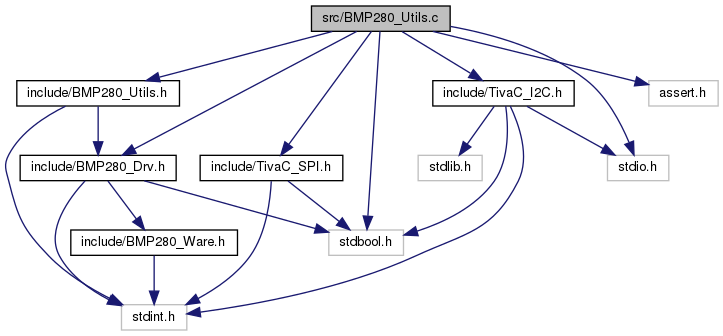
\includegraphics[width=350pt]{BMP280__Utils_8c__incl}
\end{center}
\end{figure}
\subsection*{Functions}
\begin{DoxyCompactItemize}
\item 
\mbox{\Hypertarget{BMP280__Utils_8c_a36f6ebcb6c407ee4e48a741bc77b580e}\label{BMP280__Utils_8c_a36f6ebcb6c407ee4e48a741bc77b580e}} 
\hyperlink{BMP280__Drv_8h_a726300a3932e443ece00fcc5c4f3ca7c}{Bmp280\+Err\+Code} \hyperlink{BMP280__Utils_8c_a36f6ebcb6c407ee4e48a741bc77b580e}{bmp280\+\_\+check\+\_\+setting} (\hyperlink{BMP280__Drv_8h_ab9e22f3267ce8af4053eb1189db84627}{bmp280} $\ast$sensor)
\begin{DoxyCompactList}\small\item\em check user settings to make sure they are among the supported options \end{DoxyCompactList}\item 
\mbox{\Hypertarget{BMP280__Utils_8c_a17288e03b956c789447940fb2ea10c88}\label{BMP280__Utils_8c_a17288e03b956c789447940fb2ea10c88}} 
\hyperlink{BMP280__Drv_8h_a726300a3932e443ece00fcc5c4f3ca7c}{Bmp280\+Err\+Code} \hyperlink{BMP280__Utils_8c_a17288e03b956c789447940fb2ea10c88}{bmp280\+\_\+port\+\_\+check} (\hyperlink{BMP280__Drv_8h_ab9e22f3267ce8af4053eb1189db84627}{bmp280} $\ast$sensor)
\begin{DoxyCompactList}\small\item\em port check that are run before data communication \end{DoxyCompactList}\item 
\mbox{\Hypertarget{BMP280__Utils_8c_a651c00a3684abdf07d2573d92fe45b63}\label{BMP280__Utils_8c_a651c00a3684abdf07d2573d92fe45b63}} 
\hyperlink{BMP280__Drv_8h_a726300a3932e443ece00fcc5c4f3ca7c}{Bmp280\+Err\+Code} \hyperlink{BMP280__Utils_8c_a651c00a3684abdf07d2573d92fe45b63}{bmp280\+\_\+make\+\_\+ctrl\+\_\+byte} (\hyperlink{BMP280__Drv_8h_ab9e22f3267ce8af4053eb1189db84627}{bmp280} $\ast$sensor, uint8\+\_\+t $\ast$control\+Byte)
\begin{DoxyCompactList}\small\item\em create a byte corresponding to user option to be sent to the control register on the B\+M\+P280 \end{DoxyCompactList}\item 
\mbox{\Hypertarget{BMP280__Utils_8c_a4045241afbda61ce8354f7cbb25539bc}\label{BMP280__Utils_8c_a4045241afbda61ce8354f7cbb25539bc}} 
uint8\+\_\+t \hyperlink{BMP280__Utils_8c_a4045241afbda61ce8354f7cbb25539bc}{bmp280\+\_\+make\+\_\+cfg\+\_\+byte} (\hyperlink{BMP280__Drv_8h_ab9e22f3267ce8af4053eb1189db84627}{bmp280} $\ast$sensor, uint8\+\_\+t $\ast$return\+Byte)
\begin{DoxyCompactList}\small\item\em create a byte corresponding to user option to be sent to the config register on the B\+M\+P280 \end{DoxyCompactList}\item 
\mbox{\Hypertarget{BMP280__Utils_8c_a063d98e3e3b84c4c2816ff82e4c2aacd}\label{BMP280__Utils_8c_a063d98e3e3b84c4c2816ff82e4c2aacd}} 
\hyperlink{BMP280__Drv_8h_a726300a3932e443ece00fcc5c4f3ca7c}{Bmp280\+Err\+Code} \hyperlink{BMP280__Utils_8c_a063d98e3e3b84c4c2816ff82e4c2aacd}{bmp280\+\_\+open\+\_\+i2c\+\_\+spi} (\hyperlink{BMP280__Drv_8h_ab9e22f3267ce8af4053eb1189db84627}{bmp280} $\ast$sensor)
\begin{DoxyCompactList}\small\item\em open spi or i2c communications \end{DoxyCompactList}\item 
\mbox{\Hypertarget{BMP280__Utils_8c_a3475b11b628b6248e6848694d4450450}\label{BMP280__Utils_8c_a3475b11b628b6248e6848694d4450450}} 
\hyperlink{BMP280__Drv_8h_a726300a3932e443ece00fcc5c4f3ca7c}{Bmp280\+Err\+Code} \hyperlink{BMP280__Utils_8c_a3475b11b628b6248e6848694d4450450}{bmp280\+\_\+close\+\_\+i2c\+\_\+spi} (\hyperlink{BMP280__Drv_8h_ab9e22f3267ce8af4053eb1189db84627}{bmp280} $\ast$sensor)
\begin{DoxyCompactList}\small\item\em close i2c or spi communications \end{DoxyCompactList}\item 
\mbox{\Hypertarget{BMP280__Utils_8c_a98f791b4ff6fcabbe466bbfabf0cb8f5}\label{BMP280__Utils_8c_a98f791b4ff6fcabbe466bbfabf0cb8f5}} 
\hyperlink{BMP280__Drv_8h_a726300a3932e443ece00fcc5c4f3ca7c}{Bmp280\+Err\+Code} \hyperlink{BMP280__Utils_8c_a98f791b4ff6fcabbe466bbfabf0cb8f5}{bmp280\+\_\+port\+\_\+prep} (\hyperlink{BMP280__Drv_8h_ab9e22f3267ce8af4053eb1189db84627}{bmp280} $\ast$sensor)
\begin{DoxyCompactList}\small\item\em things to run to prep the i2c/spi port for communication \end{DoxyCompactList}\item 
\mbox{\Hypertarget{BMP280__Utils_8c_a0b70b2b744d683d210f703a83cac2e6c}\label{BMP280__Utils_8c_a0b70b2b744d683d210f703a83cac2e6c}} 
\hyperlink{BMP280__Drv_8h_a726300a3932e443ece00fcc5c4f3ca7c}{Bmp280\+Err\+Code} \hyperlink{BMP280__Utils_8c_a0b70b2b744d683d210f703a83cac2e6c}{bmp280\+\_\+get\+\_\+register} (\hyperlink{BMP280__Drv_8h_ab9e22f3267ce8af4053eb1189db84627}{bmp280} $\ast$sensor, const uint8\+\_\+t start\+Addr, uint8\+\_\+t $\ast$reg\+Data, const uint8\+\_\+t total\+Register)
\begin{DoxyCompactList}\small\item\em protocol agnostic function to get data from one or multiple register \end{DoxyCompactList}\item 
\mbox{\Hypertarget{BMP280__Utils_8c_a32b99e7c569d0b4e0aa6829994041171}\label{BMP280__Utils_8c_a32b99e7c569d0b4e0aa6829994041171}} 
\hyperlink{BMP280__Drv_8h_a726300a3932e443ece00fcc5c4f3ca7c}{Bmp280\+Err\+Code} \hyperlink{BMP280__Utils_8c_a32b99e7c569d0b4e0aa6829994041171}{bmp280\+\_\+write\+\_\+register} (\hyperlink{BMP280__Drv_8h_ab9e22f3267ce8af4053eb1189db84627}{bmp280} $\ast$sensor, const uint8\+\_\+t $\ast$register\+List, const uint8\+\_\+t total\+Register, const uint8\+\_\+t $\ast$register\+Data\+List)
\begin{DoxyCompactList}\small\item\em protocol agnostic function to write data to one or multiple register \end{DoxyCompactList}\end{DoxyCompactItemize}


\subsection{Detailed Description}
Utils files contain helper functions for \hyperlink{BMP280__Drv_8c}{B\+M\+P280\+\_\+\+Drv.\+c} files as well as the glues to work with I2C and S\+PI specific stuffs. 

\begin{DoxyAuthor}{Author}
Khoi Trinh 
\end{DoxyAuthor}
\begin{DoxyDate}{Date}
2018-\/08-\/25 
\end{DoxyDate}

\hypertarget{BMP280__Ware_8c}{}\section{src/\+B\+M\+P280\+\_\+\+Ware.c File Reference}
\label{BMP280__Ware_8c}\index{src/\+B\+M\+P280\+\_\+\+Ware.\+c@{src/\+B\+M\+P280\+\_\+\+Ware.\+c}}


Contain A\+PI adapted from Bosch official source code.  


{\ttfamily \#include \char`\"{}include/\+B\+M\+P280\+\_\+\+Ware.\+h\char`\"{}}\newline
{\ttfamily \#include $<$stdint.\+h$>$}\newline
Include dependency graph for B\+M\+P280\+\_\+\+Ware.\+c\+:\nopagebreak
\begin{figure}[H]
\begin{center}
\leavevmode
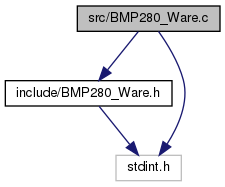
\includegraphics[width=241pt]{BMP280__Ware_8c__incl}
\end{center}
\end{figure}
\subsection*{Functions}
\begin{DoxyCompactItemize}
\item 
float \hyperlink{BMP280__Ware_8c_a24ab06b291bca8b769bab1885ff6c84d}{bmp280\+\_\+compensate\+\_\+\+T\+\_\+int32} (int32\+\_\+t adc\+\_\+T, \hyperlink{structBmp280CalibParam}{Bmp280\+Calib\+Param} $\ast$cal\+Data)
\begin{DoxyCompactList}\small\item\em calculate the temperature from B\+M\+P280 raw data \end{DoxyCompactList}\item 
float \hyperlink{BMP280__Ware_8c_a4d67cf627e8f18f614177116afe8b720}{bmp280\+\_\+compensate\+\_\+\+P\+\_\+int64} (int32\+\_\+t adc\+\_\+P, \hyperlink{structBmp280CalibParam}{Bmp280\+Calib\+Param} $\ast$cal\+Data)
\begin{DoxyCompactList}\small\item\em calculate pressure from B\+M\+P280 raw data \end{DoxyCompactList}\item 
int8\+\_\+t \hyperlink{BMP280__Ware_8c_aedbae89640aa805ae3344448b76b830f}{bmp280\+\_\+get\+\_\+calib\+\_\+param} (uint8\+\_\+t $\ast$raw\+Calib\+Data, \hyperlink{structBmp280CalibParam}{Bmp280\+Calib\+Param} $\ast$output\+Param)
\begin{DoxyCompactList}\small\item\em obtain factory calibration data from B\+M\+P280 \end{DoxyCompactList}\end{DoxyCompactItemize}


\subsection{Detailed Description}
Contain A\+PI adapted from Bosch official source code. 

\begin{DoxyDate}{Date}
2018-\/08-\/25 
\end{DoxyDate}


\subsection{Function Documentation}
\mbox{\Hypertarget{BMP280__Ware_8c_a4d67cf627e8f18f614177116afe8b720}\label{BMP280__Ware_8c_a4d67cf627e8f18f614177116afe8b720}} 
\index{B\+M\+P280\+\_\+\+Ware.\+c@{B\+M\+P280\+\_\+\+Ware.\+c}!bmp280\+\_\+compensate\+\_\+\+P\+\_\+int64@{bmp280\+\_\+compensate\+\_\+\+P\+\_\+int64}}
\index{bmp280\+\_\+compensate\+\_\+\+P\+\_\+int64@{bmp280\+\_\+compensate\+\_\+\+P\+\_\+int64}!B\+M\+P280\+\_\+\+Ware.\+c@{B\+M\+P280\+\_\+\+Ware.\+c}}
\subsubsection{\texorpdfstring{bmp280\+\_\+compensate\+\_\+\+P\+\_\+int64()}{bmp280\_compensate\_P\_int64()}}
{\footnotesize\ttfamily float bmp280\+\_\+compensate\+\_\+\+P\+\_\+int64 (\begin{DoxyParamCaption}\item[{int32\+\_\+t}]{adc\+\_\+P,  }\item[{\hyperlink{structBmp280CalibParam}{Bmp280\+Calib\+Param} $\ast$}]{cal\+Data }\end{DoxyParamCaption})}



calculate pressure from B\+M\+P280 raw data 


\begin{DoxyParams}{Parameters}
{\em adc\+\_\+P} & raw pressure data from B\+M\+P280 \\
\hline
{\em cal\+Data} & B\+M\+P280 calibration data, should be specific to each sensor due to factory manufacturing \\
\hline
\end{DoxyParams}
\begin{DoxyReturn}{Returns}
Returns pressure in Pa as unsigned 32 bit integer in Q24.\+8 format (24 integer bits and 8 fractional bits). Output value of “24674867” represents 24674867/256 = 96386.\+2 Pa = 963.\+862 h\+Pa 
\end{DoxyReturn}
\mbox{\Hypertarget{BMP280__Ware_8c_a24ab06b291bca8b769bab1885ff6c84d}\label{BMP280__Ware_8c_a24ab06b291bca8b769bab1885ff6c84d}} 
\index{B\+M\+P280\+\_\+\+Ware.\+c@{B\+M\+P280\+\_\+\+Ware.\+c}!bmp280\+\_\+compensate\+\_\+\+T\+\_\+int32@{bmp280\+\_\+compensate\+\_\+\+T\+\_\+int32}}
\index{bmp280\+\_\+compensate\+\_\+\+T\+\_\+int32@{bmp280\+\_\+compensate\+\_\+\+T\+\_\+int32}!B\+M\+P280\+\_\+\+Ware.\+c@{B\+M\+P280\+\_\+\+Ware.\+c}}
\subsubsection{\texorpdfstring{bmp280\+\_\+compensate\+\_\+\+T\+\_\+int32()}{bmp280\_compensate\_T\_int32()}}
{\footnotesize\ttfamily float bmp280\+\_\+compensate\+\_\+\+T\+\_\+int32 (\begin{DoxyParamCaption}\item[{int32\+\_\+t}]{adc\+\_\+T,  }\item[{\hyperlink{structBmp280CalibParam}{Bmp280\+Calib\+Param} $\ast$}]{cal\+Data }\end{DoxyParamCaption})}



calculate the temperature from B\+M\+P280 raw data 

Copyright (C) 2017 -\/ 2018 Bosch Sensortec GmbH

Redistribution and use in source and binary forms, with or without modification, are permitted provided that the following conditions are met\+:

Redistributions of source code must retain the above copyright notice, this list of conditions and the following disclaimer.

Redistributions in binary form must reproduce the above copyright notice, this list of conditions and the following disclaimer in the documentation and/or other materials provided with the distribution.

Neither the name of the copyright holder nor the names of the contributors may be used to endorse or promote products derived from this software without specific prior written permission.

T\+H\+IS S\+O\+F\+T\+W\+A\+RE IS P\+R\+O\+V\+I\+D\+ED BY T\+HE C\+O\+P\+Y\+R\+I\+G\+HT H\+O\+L\+D\+E\+RS A\+ND C\+O\+N\+T\+R\+I\+B\+U\+T\+O\+RS \char`\"{}\+A\+S I\+S\char`\"{} A\+ND A\+NY E\+X\+P\+R\+E\+SS OR I\+M\+P\+L\+I\+ED W\+A\+R\+R\+A\+N\+T\+I\+ES, I\+N\+C\+L\+U\+D\+I\+NG, B\+UT N\+OT L\+I\+M\+I\+T\+ED TO, T\+HE I\+M\+P\+L\+I\+ED W\+A\+R\+R\+A\+N\+T\+I\+ES OF M\+E\+R\+C\+H\+A\+N\+T\+A\+B\+I\+L\+I\+TY A\+ND F\+I\+T\+N\+E\+SS F\+OR A P\+A\+R\+T\+I\+C\+U\+L\+AR P\+U\+R\+P\+O\+SE A\+RE D\+I\+S\+C\+L\+A\+I\+M\+ED. IN NO E\+V\+E\+NT S\+H\+A\+LL C\+O\+P\+Y\+R\+I\+G\+HT H\+O\+L\+D\+ER OR C\+O\+N\+T\+R\+I\+B\+U\+T\+O\+RS BE L\+I\+A\+B\+LE F\+OR A\+NY D\+I\+R\+E\+CT, I\+N\+D\+I\+R\+E\+CT, I\+N\+C\+I\+D\+E\+N\+T\+AL, S\+P\+E\+C\+I\+AL, E\+X\+E\+M\+P\+L\+A\+RY, OR C\+O\+N\+S\+E\+Q\+U\+E\+N\+T\+I\+AL D\+A\+M\+A\+G\+ES(I\+N\+C\+L\+U\+D\+I\+NG, B\+UT N\+OT L\+I\+M\+I\+T\+ED TO, P\+R\+O\+C\+U\+R\+E\+M\+E\+NT OF S\+U\+B\+S\+T\+I\+T\+U\+TE G\+O\+O\+DS OR S\+E\+R\+V\+I\+C\+ES; L\+O\+SS OF U\+SE, D\+A\+TA, OR P\+R\+O\+F\+I\+TS; OR B\+U\+S\+I\+N\+E\+SS I\+N\+T\+E\+R\+R\+U\+P\+T\+I\+ON) H\+O\+W\+E\+V\+ER C\+A\+U\+S\+ED A\+ND ON A\+NY T\+H\+E\+O\+RY OF L\+I\+A\+B\+I\+L\+I\+TY, W\+H\+E\+T\+H\+ER IN C\+O\+N\+T\+R\+A\+CT, S\+T\+R\+I\+CT L\+I\+A\+B\+I\+L\+I\+TY, OR T\+O\+RT (I\+N\+C\+L\+U\+D\+I\+NG N\+E\+G\+L\+I\+G\+E\+N\+CE OR O\+T\+H\+E\+R\+W\+I\+SE) A\+R\+I\+S\+I\+NG IN A\+NY W\+AY O\+UT OF T\+HE U\+SE OF T\+H\+IS S\+O\+F\+T\+W\+A\+RE, E\+V\+EN IF A\+D\+V\+I\+S\+ED OF T\+HE P\+O\+S\+S\+I\+B\+I\+L\+I\+TY OF S\+U\+CH D\+A\+M\+A\+GE

The information provided is believed to be accurate and reliable. The copyright holder assumes no responsibility for the consequences of use of such information nor for any infringement of patents or other rights of third parties which may result from its use. No license is granted by implication or otherwise under any patent or patent rights of the copyright holder. 
\begin{DoxyParams}{Parameters}
{\em adc\+\_\+T} & raw B\+M\+P280 reaiding \\
\hline
{\em cal\+Data} & B\+M\+P280 calibration data, should be specific to each sensor due to factory manufacturing \\
\hline
\end{DoxyParams}
\begin{DoxyReturn}{Returns}
Returns raw\+Calib\+Dataerature in DegC, resolution is 0.\+01 DegC. Output value of “5123” equals 51.\+23 DegC. cal\+Data-\/$>$t\+\_\+fine carries fine raw\+Calib\+Dataerature as global value 
\end{DoxyReturn}
\mbox{\Hypertarget{BMP280__Ware_8c_aedbae89640aa805ae3344448b76b830f}\label{BMP280__Ware_8c_aedbae89640aa805ae3344448b76b830f}} 
\index{B\+M\+P280\+\_\+\+Ware.\+c@{B\+M\+P280\+\_\+\+Ware.\+c}!bmp280\+\_\+get\+\_\+calib\+\_\+param@{bmp280\+\_\+get\+\_\+calib\+\_\+param}}
\index{bmp280\+\_\+get\+\_\+calib\+\_\+param@{bmp280\+\_\+get\+\_\+calib\+\_\+param}!B\+M\+P280\+\_\+\+Ware.\+c@{B\+M\+P280\+\_\+\+Ware.\+c}}
\subsubsection{\texorpdfstring{bmp280\+\_\+get\+\_\+calib\+\_\+param()}{bmp280\_get\_calib\_param()}}
{\footnotesize\ttfamily int8\+\_\+t bmp280\+\_\+get\+\_\+calib\+\_\+param (\begin{DoxyParamCaption}\item[{uint8\+\_\+t $\ast$}]{raw\+Calib\+Data,  }\item[{\hyperlink{structBmp280CalibParam}{Bmp280\+Calib\+Param} $\ast$}]{output\+Param }\end{DoxyParamCaption})}



obtain factory calibration data from B\+M\+P280 


\begin{DoxyParams}{Parameters}
{\em raw\+Calib\+Data} & calibration data read from B\+M\+P280 registers \\
\hline
{\em output\+Param} & pointer to output calibration data \\
\hline
\end{DoxyParams}

\hypertarget{main_8c}{}\section{src/main.c File Reference}
\label{main_8c}\index{src/main.\+c@{src/main.\+c}}


used for testing and also serve as an example  


{\ttfamily \#include $<$stdbool.\+h$>$}\newline
{\ttfamily \#include $<$stdio.\+h$>$}\newline
{\ttfamily \#include $<$stdlib.\+h$>$}\newline
{\ttfamily \#include \char`\"{}external/\+Tiva\+C\+\_\+\+Utils/include/\+Tiva\+C\+\_\+\+L\+E\+D.\+h\char`\"{}}\newline
{\ttfamily \#include \char`\"{}external/\+Tiva\+C\+\_\+\+Utils/include/\+Tiva\+C\+\_\+\+Other\+\_\+\+Utils.\+h\char`\"{}}\newline
{\ttfamily \#include \char`\"{}include/\+B\+M\+P280\+\_\+\+Drv.\+h\char`\"{}}\newline
{\ttfamily \#include \char`\"{}include/\+B\+M\+P280\+\_\+\+Ware.\+h\char`\"{}}\newline
{\ttfamily \#include \char`\"{}include/\+Tiva\+C\+\_\+\+I2\+C.\+h\char`\"{}}\newline
Include dependency graph for main.\+c\+:\nopagebreak
\begin{figure}[H]
\begin{center}
\leavevmode
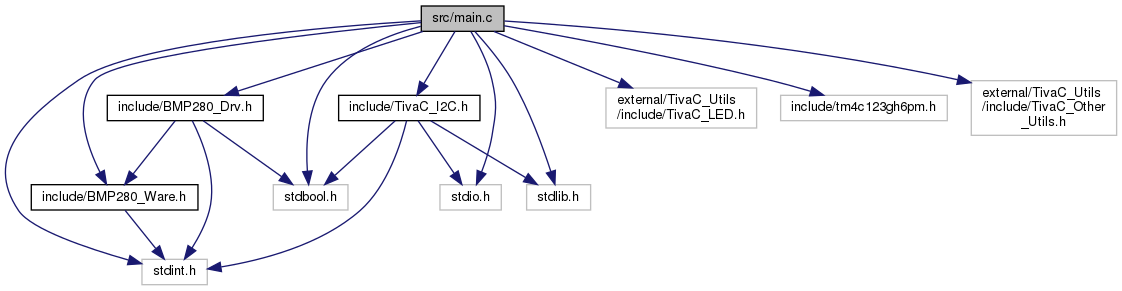
\includegraphics[width=350pt]{main_8c__incl}
\end{center}
\end{figure}
\subsection*{Macros}
\begin{DoxyCompactItemize}
\item 
\mbox{\Hypertarget{main_8c_a64daeac0e223512b505ab0caa06ddbd8}\label{main_8c_a64daeac0e223512b505ab0caa06ddbd8}} 
\#define {\bfseries B\+M\+P280\+\_\+\+A\+D\+DR}~0x77
\end{DoxyCompactItemize}
\subsection*{Functions}
\begin{DoxyCompactItemize}
\item 
\mbox{\Hypertarget{main_8c_a840291bc02cba5474a4cb46a9b9566fe}\label{main_8c_a840291bc02cba5474a4cb46a9b9566fe}} 
int {\bfseries main} (void)
\end{DoxyCompactItemize}


\subsection{Detailed Description}
used for testing and also serve as an example 

\begin{DoxyAuthor}{Author}
Khoi Trinh 
\end{DoxyAuthor}
\begin{DoxyDate}{Date}
2018-\/08-\/25 
\end{DoxyDate}

\hypertarget{TivaC__I2C_8c}{}\section{src/\+Tiva\+C\+\_\+\+I2C.c File Reference}
\label{TivaC__I2C_8c}\index{src/\+Tiva\+C\+\_\+\+I2\+C.\+c@{src/\+Tiva\+C\+\_\+\+I2\+C.\+c}}


Contain main I2C functions for T\+IvaC.  


{\ttfamily \#include \char`\"{}include/\+Tiva\+C\+\_\+\+I2\+C.\+h\char`\"{}}\newline
{\ttfamily \#include $<$stdbool.\+h$>$}\newline
{\ttfamily \#include \char`\"{}external/\+Tiva\+C\+\_\+\+Utils/include/tm4c123gh6pm.\+h\char`\"{}}\newline
Include dependency graph for Tiva\+C\+\_\+\+I2\+C.\+c\+:\nopagebreak
\begin{figure}[H]
\begin{center}
\leavevmode
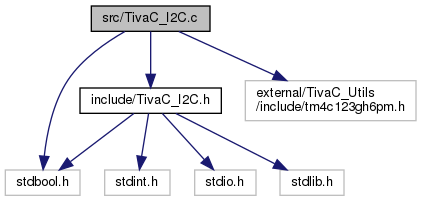
\includegraphics[width=350pt]{TivaC__I2C_8c__incl}
\end{center}
\end{figure}
\subsection*{Macros}
\begin{DoxyCompactItemize}
\item 
\mbox{\Hypertarget{TivaC__I2C_8c_a4ccb093ce990b3d0dd67ba286b5b40cf}\label{TivaC__I2C_8c_a4ccb093ce990b3d0dd67ba286b5b40cf}} 
\#define {\bfseries S\+C\+L\+\_\+\+LP}~6
\item 
\mbox{\Hypertarget{TivaC__I2C_8c_ad36d068c694b11d45af851c811e46394}\label{TivaC__I2C_8c_ad36d068c694b11d45af851c811e46394}} 
\#define {\bfseries S\+C\+L\+\_\+\+HP}~4
\item 
\mbox{\Hypertarget{TivaC__I2C_8c_a1ef39cf839b4b9aa3f018ebac932a6dd}\label{TivaC__I2C_8c_a1ef39cf839b4b9aa3f018ebac932a6dd}} 
\#define {\bfseries I2\+C0\+\_\+\+T\+I\+M\+E\+O\+U\+T\+\_\+\+L\+I\+M\+IT}~10000
\end{DoxyCompactItemize}
\subsection*{Functions}
\begin{DoxyCompactItemize}
\item 
\mbox{\Hypertarget{TivaC__I2C_8c_ab67308783773adc604bd5a0d87a511af}\label{TivaC__I2C_8c_ab67308783773adc604bd5a0d87a511af}} 
I2c0\+Err\+Code \hyperlink{TivaC__I2C_8c_ab67308783773adc604bd5a0d87a511af}{i2c0\+\_\+open} (void)
\begin{DoxyCompactList}\small\item\em enable clocks, I2C pins and calculate the appropriate clock period This function should be called first b4 any I2C operations \end{DoxyCompactList}\item 
\mbox{\Hypertarget{TivaC__I2C_8c_ad78ce9ab48b822965a2e58c0389edbd1}\label{TivaC__I2C_8c_ad78ce9ab48b822965a2e58c0389edbd1}} 
I2c0\+Err\+Code \hyperlink{TivaC__I2C_8c_ad78ce9ab48b822965a2e58c0389edbd1}{i2c0\+\_\+close} (void)
\begin{DoxyCompactList}\small\item\em Disable clock as well as the I2C pins. \end{DoxyCompactList}\item 
I2c0\+Err\+Code \hyperlink{TivaC__I2C_8c_ae51adb7272b1571ff425a124f0f5a7a5}{i2c0\+\_\+single\+\_\+data\+\_\+read} (const uint8\+\_\+t slave\+\_\+address, uint8\+\_\+t $\ast$return\+Data, const bool no\+\_\+ack, const bool no\+\_\+stop, const bool no\+\_\+start)
\begin{DoxyCompactList}\small\item\em read one byte of data \end{DoxyCompactList}\item 
I2c0\+Err\+Code \hyperlink{TivaC__I2C_8c_ab8c85ee87b4d758a3ff1bfbdbec6bf26}{i2c0\+\_\+single\+\_\+data\+\_\+write} (const uint8\+\_\+t slave\+\_\+address, const uint8\+\_\+t data\+\_\+byte, const bool no\+\_\+end\+\_\+stop)
\begin{DoxyCompactList}\small\item\em write a single byte using I2C \end{DoxyCompactList}\item 
\mbox{\Hypertarget{TivaC__I2C_8c_ab9a581a005285f7e94a5c79d956f207b}\label{TivaC__I2C_8c_ab9a581a005285f7e94a5c79d956f207b}} 
I2c0\+Err\+Code \hyperlink{TivaC__I2C_8c_ab9a581a005285f7e94a5c79d956f207b}{i2c0\+\_\+stop} (void)
\begin{DoxyCompactList}\small\item\em used to generate I2C stop signal \end{DoxyCompactList}\item 
\mbox{\Hypertarget{TivaC__I2C_8c_ad6ba2e0d794a585e8f69ea37033971fa}\label{TivaC__I2C_8c_ad6ba2e0d794a585e8f69ea37033971fa}} 
I2c0\+Err\+Code \hyperlink{TivaC__I2C_8c_ad6ba2e0d794a585e8f69ea37033971fa}{i2c0\+\_\+keep\+\_\+state} (void)
\begin{DoxyCompactList}\small\item\em used to maintain current I2C state \end{DoxyCompactList}\item 
\mbox{\Hypertarget{TivaC__I2C_8c_af0bd7f3c3b91870a3b7616dd5d848365}\label{TivaC__I2C_8c_af0bd7f3c3b91870a3b7616dd5d848365}} 
I2c0\+Err\+Code \hyperlink{TivaC__I2C_8c_af0bd7f3c3b91870a3b7616dd5d848365}{i2c0\+\_\+multiple\+\_\+data\+\_\+byte\+\_\+write} (const uint8\+\_\+t slave\+\_\+address, const uint8\+\_\+t $\ast$output\+\_\+buffer, const uint8\+\_\+t output\+\_\+buffer\+\_\+length)
\begin{DoxyCompactList}\small\item\em write byte one by one until done \end{DoxyCompactList}\item 
\mbox{\Hypertarget{TivaC__I2C_8c_a8e258129956544f01ec903e3dd153454}\label{TivaC__I2C_8c_a8e258129956544f01ec903e3dd153454}} 
I2c0\+Err\+Code {\bfseries i2c0\+\_\+multiple\+\_\+data\+\_\+byte\+\_\+read} (const uint8\+\_\+t slave\+\_\+address, uint8\+\_\+t $\ast$input\+\_\+buffer, const uint8\+\_\+t input\+\_\+buffer\+\_\+length)
\item 
\mbox{\Hypertarget{TivaC__I2C_8c_ab0f051ca77472369ee6bbb68b020f657}\label{TivaC__I2C_8c_ab0f051ca77472369ee6bbb68b020f657}} 
I2c0\+Err\+Code \hyperlink{TivaC__I2C_8c_ab0f051ca77472369ee6bbb68b020f657}{i2c0\+\_\+error\+\_\+check} (void)
\begin{DoxyCompactList}\small\item\em check i2c error register for any problems \end{DoxyCompactList}\item 
\mbox{\Hypertarget{TivaC__I2C_8c_a8cb69d8095fdbe6d8447f3413c280e03}\label{TivaC__I2C_8c_a8cb69d8095fdbe6d8447f3413c280e03}} 
I2c0\+Err\+Code \hyperlink{TivaC__I2C_8c_a8cb69d8095fdbe6d8447f3413c280e03}{i2c0\+\_\+check\+\_\+master\+\_\+enabled} (void)
\begin{DoxyCompactList}\small\item\em check i2c config register to see if the master functionality is enabled \end{DoxyCompactList}\item 
I2c0\+Err\+Code \hyperlink{TivaC__I2C_8c_ade2063cad2d3a4744d325dbbb3eda2c4}{i2c0\+\_\+wait\+\_\+bus} (void)
\begin{DoxyCompactList}\small\item\em used for waiting till the bus stops being busy \end{DoxyCompactList}\end{DoxyCompactItemize}


\subsection{Detailed Description}
Contain main I2C functions for T\+IvaC. 

\begin{DoxyAuthor}{Author}
Khoi Trinh 
\end{DoxyAuthor}
\begin{DoxyDate}{Date}
2018-\/08-\/25 
\end{DoxyDate}


\subsection{Function Documentation}
\mbox{\Hypertarget{TivaC__I2C_8c_ae51adb7272b1571ff425a124f0f5a7a5}\label{TivaC__I2C_8c_ae51adb7272b1571ff425a124f0f5a7a5}} 
\index{Tiva\+C\+\_\+\+I2\+C.\+c@{Tiva\+C\+\_\+\+I2\+C.\+c}!i2c0\+\_\+single\+\_\+data\+\_\+read@{i2c0\+\_\+single\+\_\+data\+\_\+read}}
\index{i2c0\+\_\+single\+\_\+data\+\_\+read@{i2c0\+\_\+single\+\_\+data\+\_\+read}!Tiva\+C\+\_\+\+I2\+C.\+c@{Tiva\+C\+\_\+\+I2\+C.\+c}}
\subsubsection{\texorpdfstring{i2c0\+\_\+single\+\_\+data\+\_\+read()}{i2c0\_single\_data\_read()}}
{\footnotesize\ttfamily I2c0\+Err\+Code i2c0\+\_\+single\+\_\+data\+\_\+read (\begin{DoxyParamCaption}\item[{const uint8\+\_\+t}]{slave\+\_\+address,  }\item[{uint8\+\_\+t $\ast$}]{return\+Data,  }\item[{const bool}]{no\+\_\+ack,  }\item[{const bool}]{no\+\_\+stop,  }\item[{const bool}]{no\+\_\+start }\end{DoxyParamCaption})}



read one byte of data 


\begin{DoxyParams}{Parameters}
{\em no\+\_\+ack} & whether to generate ack signal \\
\hline
{\em no\+\_\+stop} & whether to generate stop signal \\
\hline
{\em no\+\_\+start} & whether to generate start(or repeated start) signal \\
\hline
\end{DoxyParams}
\mbox{\Hypertarget{TivaC__I2C_8c_ab8c85ee87b4d758a3ff1bfbdbec6bf26}\label{TivaC__I2C_8c_ab8c85ee87b4d758a3ff1bfbdbec6bf26}} 
\index{Tiva\+C\+\_\+\+I2\+C.\+c@{Tiva\+C\+\_\+\+I2\+C.\+c}!i2c0\+\_\+single\+\_\+data\+\_\+write@{i2c0\+\_\+single\+\_\+data\+\_\+write}}
\index{i2c0\+\_\+single\+\_\+data\+\_\+write@{i2c0\+\_\+single\+\_\+data\+\_\+write}!Tiva\+C\+\_\+\+I2\+C.\+c@{Tiva\+C\+\_\+\+I2\+C.\+c}}
\subsubsection{\texorpdfstring{i2c0\+\_\+single\+\_\+data\+\_\+write()}{i2c0\_single\_data\_write()}}
{\footnotesize\ttfamily I2c0\+Err\+Code i2c0\+\_\+single\+\_\+data\+\_\+write (\begin{DoxyParamCaption}\item[{const uint8\+\_\+t}]{slave\+\_\+address,  }\item[{const uint8\+\_\+t}]{data\+\_\+byte,  }\item[{const bool}]{no\+\_\+end\+\_\+stop }\end{DoxyParamCaption})}



write a single byte using I2C 


\begin{DoxyParams}{Parameters}
{\em no\+\_\+end\+\_\+stop} & whether to generate stop at the end of the write \\
\hline
\end{DoxyParams}
\mbox{\Hypertarget{TivaC__I2C_8c_ade2063cad2d3a4744d325dbbb3eda2c4}\label{TivaC__I2C_8c_ade2063cad2d3a4744d325dbbb3eda2c4}} 
\index{Tiva\+C\+\_\+\+I2\+C.\+c@{Tiva\+C\+\_\+\+I2\+C.\+c}!i2c0\+\_\+wait\+\_\+bus@{i2c0\+\_\+wait\+\_\+bus}}
\index{i2c0\+\_\+wait\+\_\+bus@{i2c0\+\_\+wait\+\_\+bus}!Tiva\+C\+\_\+\+I2\+C.\+c@{Tiva\+C\+\_\+\+I2\+C.\+c}}
\subsubsection{\texorpdfstring{i2c0\+\_\+wait\+\_\+bus()}{i2c0\_wait\_bus()}}
{\footnotesize\ttfamily I2c0\+Err\+Code i2c0\+\_\+wait\+\_\+bus (\begin{DoxyParamCaption}\item[{void}]{ }\end{DoxyParamCaption})}



used for waiting till the bus stops being busy 

\begin{DoxyReturn}{Returns}
whether the bus is idle now or timeout happened 
\end{DoxyReturn}

%--- End generated contents ---

% Index
\backmatter
\newpage
\phantomsection
\clearemptydoublepage
\addcontentsline{toc}{chapter}{Index}
\printindex

\end{document}
